%\graphicspath{{13-procex/small_images/}}
\graphicspath{{13-procex/images/}}

\chapter{Procedural Extrusions}
\label{c:procex}

\greybox{This section is based on the paper \emph{Interactive Architectural Modeling with Procedural Extrusions}\cite{twak11}, co-authored with Peter Wonka.}


%-------------------------------------------------------------------------
\section{Introduction}



Given the contribution of the skeleton to the success of modeling city block subdivision, a natural question is to ask which other urban domains it may contribute to the modeling of? 

Recall again the urban procedural modeling pipeline of Fig.~\ref{fig:umPipeline}, in which streets subdivide land into blocks, algorithms such as those in the previous chapter divide the blocks into parcels, parcels are converted to footprints, and footprints are used to create mass models of buildings. Here we are interested in the final stage of this waterfall pipeline, creating solid 3D buildings from 2D footprints. To do this procedurally, that is for an arbitrary footprint or plan, without programming is the challenge we address here. To approach this problem we take inspiration from artists' plan and elevation drawings, and the flexibility of the mixed weighted straight skeleton of Chapter 3. The combination of these techniques allows us to interactively create robust 3D procedural models parameterised by the footprints. 



We introduce an application of the MWSS to the interactive procedural modeling of architectural forms. The \emph{procedural extrusion} (PE) system procedurally generates solid 3D meshes by extruding building footprints. Such an application of the straight skeleton to the creation of architectural surfaces allows for the generation of difficult architectural surfaces such as curved roofs, overhanging roofs, dormer windows, interior dormer windows, roof constructions with vertical walls, buttresses, chimneys, bay windows, columns, pilasters, and alcoves. The system comprises of a user interface to specify procedural extrusions manually as well as a tool for the automated generation of large procedural cityscapes from their footprints. Extensions to the the sweep plane algorithm of Chapter~\ref{c:various_skels} are utilised to robustly compute a wide range of two-manifold architectural surfaces.


The procedural extrusion system is both an interactive and procedural modeling tool for such architectural surfaces. Procedural geometric modeling offers several advantages over traditional static modeling of architectural forms. PGM descriptions of objects allow us to edit meshes at a higher semantic level; for example, editing wall angles rather than vertex coordinates, whilst ensuring constraints are enforced, such as polygon planarity. Additionally we can preserve subsequent edits while allowing earlier edits to be modified; such as changing the slope of a roof after a chimney has been created upon it, without adjusting the chimney. Nevertheless, the biggest advantage of procedural modeling over static modeling is the creation of large scale cityscapes, without a proportional increase in designer effort. Many of the current PGM systems, such as CGA Shape\cite{Pascal06}, require end user programming. In contrast, the PE system provides an interactive graphical tool, instead of a programming language, to specify geometry. This lowers the barriers of entry to PGM, allowing more people to create procedural content.

\begin{figure}
  \centering
  \includegraphics[width=1.0\columnwidth]{SingleHouse.png}
  \caption[A house created using procedural extrusions.]{\label{fig:SingleHouse}
Procedural extrusions allow a footprint (2d plan) to be extruded to form the walls and roof of a house (inset). Meshes and procedural details can then be attached (main).}
\end{figure}

Architectural surfaces are often deeply concave and contain complex architectural features such as overhanging roofs, dormer windows, interior dormer windows, roof constructions with vertical walls, buttresses, chimneys, bay windows, columns, pilasters, and alcoves. These intricate surfaces have not previously been available as watertight meshes in procedural environments. Systems such as shape grammars\cite{Stiny80,Mueller:2006:PMB,Lipp:2008:IEV} have tended to concentrate on the combinatorial, rather than the geometric aspects of architecture generation, and are not able to generate such geometry themselves. Typically these systems rely on pre-existing meshes that are instanced, positioned, and scaled to appropriate locations.

Given buildings, such as in Fig.~\ref{fig:two_profiles}, it is not obvious how to construct 3D models of these structures. Procedural extrusions provide a novel parametrisation of such buildings by taking inspiration from architects' drawings consisting of floorplans and elevations. 

\begin{figure}
  \centering
  \def\svgwidth{1.0\columnwidth}
  \includesvg{13-procex/images/two_profiles}
  \caption[Plans and profiles of two architectural models]{\label{fig:two_profiles}
  These two examples show architectural surfaces overlayed with the user input. Plans (green), profiles (blue), natural steps (orange) and offset events (red) are specified in the user interface. The output of our system is an architectural shell (grey). }
\end{figure}

The first major component of the system is presented in Sec.~\ref{sec:UI} and allows the user to interactively draw a floorplan, and assign an arbitrary profiles to each plan edge. Nested sets of plans and profiles allow features such as dormer windows and alcoves (Fig.~\ref{fig:two_profiles}, orange) to be modeled. Interactive modeling via the user interface allows the expressiveness of the system to be explored in depth. We evaluate the interactive portion of the PE system in Sec.~\ref{Sec:Evaluation} by modeling $50$ various structures from a catalogue, as well as seeking opinions from users as to the properties of the system.

In order to combine arbitrary plans and profiles, the second component of the system is a collection of algorithms to construct 3D meshes from the specified plans and profiles. These algorithms utilise a variety of repeated applications of the MWSS (Chapter~\ref{c:various_skels}, Sec.~\ref{sec:mwss}) to create a geometry modeling system. We take the sweep-plane that is used to calculate the MWSS and introduce additional types of user specified events. These algorithms are presented in Sec.~\ref{sec:method}. To study the real-world stability of these algorithms we evaluate PEs over a large scale data of $6000$ building footprints in Sec.~\ref{Sec:Evaluation}. Here we note that the computational geometry community emphasises provably correct algorithms and therefore often favours rational arithmetic. In contrast, our work consists of heuristic algorithms that emphasise computational speed and are geared towards a floating point implementation. While our heuristics include various mechanisms to make the results more robust, it is possible that the computations can fail. For example, in the Atlanta data set of $6000$ footprints we noted that two roof planes were not computed correctly. The approximate nature of our floating point computation also results in roof planes being moved by millimetres.

We conclude  with a description of external applications to which others have successfully applied components of the PE system.

The contributions of our work are:
\begin{itemize}
\item the design of the system and tools to enable procedural modeling of complex architectural surfaces.
\item the set of tool choices to enable procedural modeling of complex architectural surfaces.
\item heuristic algorithms to generate a polygonal mesh from the user specification that is approximately consistent with the input data.
\item the evaluation of the system on a collection of examples to verify its practical utility, and to identify configurations that are difficult to model with our tools.
\end{itemize}


%-------------------------------------------------------------------------
\section{Related work}
%\section{Similar Techniques}
\label{sec:alternatives}

In this section we describe and examine some common techniques applied to architectural modeling and analyse some of the properties of the resulting architectural meshes. 

We may make the observation that many architectural and man-made objects have a common property: \emph{There are many horizontal edges to the geometry, and the faces between such edges are rectangular and coplanar}. For example Fig.~\ref{fig:horiz_lines} shows one building with many horizontal edges and associated faces.

\begin{figure}
  \centering
  \def\svgwidth{1.0\columnwidth}
  \includesvg{13-procex/images/horiz_lines}
  \caption[Horizontal edges are common in architectural form]{\label{fig:horiz_lines}In many buildings' geometries, there are many horizontal edges (green). Many faces of such geometry are coplanar to one or two such edges. In this case, only the red faces do not do not have such a horizontal edge.}
\end{figure}

There are several properties that we find desirable in computer models of architectural structures. We assume to use polygonal mesh models, since these are common, somewhat standard in industry, and are those which hardware (GPU) acceleration is designed to accommodate. ``Nice'' 3D meshes commonly have the following properties: 
\begin{itemize}
\item{Planar faces: Each face lies entirely within a single plane.}
\item{Water-tight: There are no holes in the mesh, all adjacent faces are connected via a shared edge, and all adjacent edges are connected via a shared vertex.}
\item{No self-intersections: No part of the mesh protrudes through another; the only parts of the mesh that touch are adjacent in the mesh data structure.}
\end{itemize} 

\begin{figure}
  \centering
  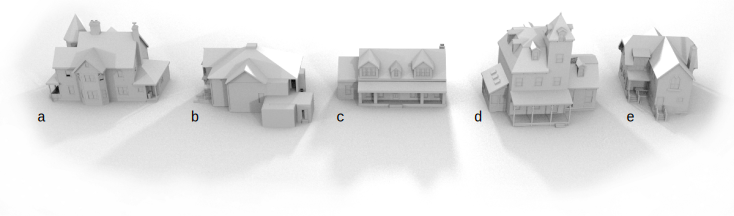
\includegraphics[width=1.0\columnwidth]{googleWarehouseComp.png}
  \caption[Examples of buildings modeled in Sketchup]{\label{fig:googleWarehouseComp} Several typical building meshes created using Sketchup\cite{Sketchup}, and found in Trimble Warehouse\cite{GoogleWarehouse} using the search ``Victorian house''. From left to right the buildings were created by users wiccan, DILBERT, bob1938, Paulwall and bob1938. Buildings have had garden geometry and textures removed to allow comparison with our results. \copyright 2013 Google.}
\end{figure}


To describe such meshes, basic 3D modeling tools such as as those introduced in Sec.~\ref{sec:construction} may be used. Tools such as manual vertex modeling, extrusion, lofting, and constructive solid geometry have all been used to model architecture in 3D modeling tools such as Maya\cite{Maya}, Sketchup\cite{Sketchup}, and Blender\cite{Blender}. Several examples of buildings created with the Sketchup modeling tool are shown in Fig.~\ref{fig:googleWarehouseComp}.


\begin{itemize}

\item{Manual vertex and face specification gives users the tools to create and position verticies in $\mathbb{R}^3$. These tools allow unrestricted mesh creation, but it is possible, and even common, for such tools to create non-planar polygons, non-watertight, or self-intersecting meshes. Often additional post-processing stages must be applied to check for these conditions, and resolving them is left to the user. Fig.~\ref{fig:vertex_edit} illustrates how moving a single vertex may result in several non-planar faces.}

\begin{figure}
  \centering
  \def\svgwidth{0.7\columnwidth}
  \includesvg{13-procex/images/mesh_edit}
  \caption[Mesh editing may not preserve face planarity.]{\label{fig:vertex_edit}Given a mesh (left), translating a single point(orange) may result in one or more non-planar faces(right).}
\end{figure}

\item{Extruding a plan-polygon either in a single direction or along a 3D path, Fig.~\ref{fig:Extrude}, left, is another method to construct meshes with rectangular faces. Careful positioning of the plan and profile can produce meshes with the desired horizontal edge property. An extrusion tool creates an instance of the plan at each vertex of the path. It continues to create a rectangular face between the pairs of corresponding plan edges from adjacent plan-instances. 

However there are some problems with the extrusion tool. If the path rotates, the faces of the resulting geometry may not be planar, Fig.~\ref{fig:Extrude}, centre. Additionally, when modelling walls and roofs, the plans and profiles are not changed in response to the geometry; self-intersections may occur, such as when modeling roofs --- the crest of the roof may either fall short, or overshoot as in Fig.~\ref{fig:Extrude}, right. Such deficiencies with geometry created by the extrude tool must be identified and removed manually, possible with manual vertex and face edits.

\emph{Levelshop}\cite{Fong11} is a rapid video game level prototyping tool that uses extrusions, together with user defined 2D plans. Because of the above problems with extrusion, it is limited to relatively simple geometry.}

\begin{figure}
  \centering
  \def\svgwidth{1.0\columnwidth}
  \includesvg{13-procex/images/extrude}
  \caption[Failure cases with extrude tool]{\label{fig:Extrude}Left: A plan polygon (green) is extruded along a single segment path (blue). Rectangular faces are created between adjacent instances of the polygon. The above verticies $p^1_1$, $p^2_1$, from the first instance, and $p^1_2$ and $p^2_2$, from the second, form the orange rectangle. Centre: If the path rotates an instance, faces may not be planar. Note that the non-planar quads are depicted here as triangles. Right: Using a more complex path, geometry with strong horizontal lines can be created. However self-intersections and holes in the geometry are evident in this example, such as near the roof line of this mesh, and above the concavity in the plan.}
\end{figure}

\item{A modification to the extrusion algorithm allows for different profiles to be used at each vertex on the profile. This \emph{loft tool} allows more  user  interaction, so that when the geometry does self-intersect, the profiles may be manually edited. Lofts are a modeling primitive extensively used in 3D modeling packages. As when extruding there are no guarantees that the result of a loft will not self-intersect. The manual editing of profiles can be quite involved as it requires the user to specify additional segments for some of the polyline instances as well as specifying corresponding topologies for face creation.}

\item{Another popular method for geometry creation is \emph{constructive solid geometry}\cite{Atherton83} to form objects from the addition and subtraction of geometry elements. CSG has been used by several systems since to create urban modeling tools. Sugihara and Hayashi\cite{Sugihara08} create roofs on orthogonal geometry by unioning roofs after rectangular decomposition. This approach is adapted to building reconstruction in~\cite{Lafarge10}, by computing the CSG union of elements from a library of 3D roof-form blocks.

The advantages of CSG are that manifold results are guaranteed, and that all the output faces are subsets of the input faces. Thus if the input faces are planar, then so will the result. The disadvantage is, however, that the range of results are limited by the available CSG primitives, as illustrated in Fig.~\ref{fig:csg}.}
\end{itemize}

\begin{figure}
  \centering
  \def\svgwidth{1.0\columnwidth}
  \includesvg{13-procex/images/csg}
  \caption[CSG failure cases]{\label{fig:csg}The expressiveness of a constructive solid approach, given a single input primitive (a) is limited. For example, we may wish to elongate the primitive. A CSG union operation could only construct a mesh with several peaks (b), while a scale operation would also adjust the slope of the roof in an unrealistic manner (c), however we probably prefer a result closer to the straight skeleton (d). In a second example, the union (e) is not the same as the SS (f), and introduces unwanted, water collecting, horizontal edges into the roof-line. More complex examples (g) cannot be created at all, since they are not locally similar to the available primitive.}
\end{figure}

\FloatBarrier

As introduced in Chapter~\ref{c:readings} there are a wide range of languages and grammars for specifying geometry. Many of these systems, such as CGA Shape\cite{Pascal06}, are concerned with the combinatorial and positional aspects of the modeling, rather than the geometric elements. For example, CGA may specify the location of the roof, but would rely on extrude operations to specify the mass model and other geometric routines to calculate the roof geometry.

%Modeling packages. unlear algorithms.
%Specialist architectural modeling tools... Procedural extrusions bear a resemblance to several modeling techniques available in commercial packages. Here we outline several of these techniques in relation to archiectural shell design. \cite{Revit}\cite{AutoCAD}.

% deformation techniques
Several systems exist to deform existing architectural meshes into new configurations~\cite{Habbecke12, Cabral09, Gal09}, additional detail is given in Chapter~\ref{c:readings}. For example, in \cite{Habbecke12} Habbecke and Kobbelt introduce a mesh deformation tool that constrains specified edges to remain, for example, coplanar, horizontal or vertical. The system constructs a linear system that may be deformed in real time. These deformation tools, however, do not solve the problem of creating geometry to be deformed in the first place.

Previous systems have applied the straight skeleton to the modeling of architectural roofs. Laycock and Day\cite{Laycock03} use the SS to define roofs over arbitrary floorplans, and adjust the positions of the verticies to create Gable roofs. Havemann\cite{Havemann:2005:GMM} uses an application of the SS with uniform negative weights, followed by an application with uniform positive weights to create overhanging roofs. Our goals are similar to these approaches and we contribute new extensions to the straight skeleton to avoid the need for Laycock's vertex adjustment and to extend the skeleton beyond roof modeling to an interactive procedural modeling system for entire architectural meshes.



\begin{figure}
  \centering
  \def\svgwidth{0.6\columnwidth}
  \includesvg{13-procex/images/vsmedial}
  \caption[Modeling building roofs with the medial axis.]{\label{fig:vsmedial}A comparison of modeling roofs with the medial axis, left, and the straight skeleton, right. The corresponding 2D geometries are shown above.}
\end{figure}

An alternative to the SS for offsetting areas is the medial axis\cite{Blum67}. As discussed in Sec.~\ref{sec:skeletonSubivision}, there are several technical limitations to using the medial axis in the polygonal domain. In addition we may wish to study the aesthetic reasons for not using the medial axis; we can ignore these technical limitations to create a model such as demonstrated in Fig.~\ref{fig:vsmedial}. In this model we observe that there are many unrealistic curved roof ridges, both when viewing the model from the top or the sides. These unrealistic curved edges make the medial axis much less suitable for modeling the roofs of buildings than the straight skeleton. In addition we note that the method used to visualise the medial axis for Fig.~\ref{fig:vsmedial} created 65,000 polygons, compared to the 80 polygons created by the SS algorithm. This large difference in model complexity was caused by the terrain used to model the roof from a 2D bitmap image of a medial axis computation. It may be possible to create such 3D models using the medial axis with fewer polygons, but we are unaware of any such published techniques.


%%-------------------------------------------------------------------------
%%
\section{User Interface Description}
\label{sec:UI}

To control the underlying application of MWSS instances, the PE system utilises a graphical user interface. This section introduces the interface, and how it can be used to model single instances of complex watertight architectural meshes, we call \emph{shells}. The MWSS algorithms are largely motivated by the desirable user interface commands, and so the user interface provides a motivation for the technicalities in the following sections. These new event types specified by the UI are explained in Sec.~\ref{sec:WSS}.

\subsection {Overview}
\label{sec:UI:overview}

Our UI originates from the observation that simple roofs can be defined by a aerial plan, and an angle for the roof. We combined this line of enquiry with the study of architect's drawings that combine plan drawings from above, and elevation images from the four sides. The plan specifies the footprint of the structure, while the observed roof angle is often present in the elevations. Exploring this observation, one may extract angles and heights from other locations on the profile in an architectural elevation, such as the height of the walls. However, architects typically produce a small number of elevations, typically one for each cardinal direction, and this provides insufficient detail for reconstruction. For example when the footprint of the house contains concavities, cardinal elevations under-constrain the resulting solid shape. The premise of the PE system is to create solid geometry from a \emph{plan} and per plan-edge \emph{profiles}, as in Fig.~\ref{fig:two_profiles}. 


\begin{figure*}
  \centering
 \def\svgwidth{1.0\columnwidth}
\includesvg{13-procex/images/ui_strip}
\caption[Example PE plans and profiles.]{\label{fig:ui_strip} Three example buildings constructed in our user interface. We demonstrate multiple profiles on a simple plan (abcd), modeling overhangs (efghi) and anchors (jklmn). Simple profiles (ab) are applied to the green and purple edges of the plan (c) to create the geometry (d). Overhangs are defined using an additional pair of profile polylines associated with every edge (ef) to create typical roof geometry (hi). Anchors (magenta circles) are defined on the profile (j) and the plan (l) to position features. In this example the anchors position a rectangular natural step (m) with a profile (k) that creates a roof-window (n).
}
\end{figure*}

The plans and profiles are evaluated by a rising sweep plane algorithm, in a manner similar MWSS, of Sec.~\ref{sec:mwss}. As the sweep plane rises, it carries with it an \emph{active plan} which combines the different profiles to create a solid polygonal mesh. 


The complete UI, including the MWSS implementation, is available online\cite{siteplan}.


\subsection{Plans and Profiles}

The complete user interface, as illustrated in Fig.~\ref{fig:ui} and provides:
\begin{itemize}
\item{the current plan,}
\item{the current profile,}
\item{a 3D preview of the current architectural shell,}
\item{tools to add, remove and move verticies in the plan and profile,}
\item{tools to associate profiles with plan edges,}
\item{options to add and remove profiles}
\item{options to add \emph{events} to the profile and plan using anchors. There are several different types of discrete UI events, introduced below, which are enacted as the sweep plane rises past them.}
\item{Finally the UI also provides standard save, load, and export functionality.}
\end{itemize}

\begin{figure}
  \centering
  \includegraphics[width=1.0\columnwidth]{ui.png}
  \caption[The PE GUI.]{\label{fig:ui}
The interactive interface during the design of a temple. The right window contains the output preview whilst the left window contains the plan and the profile editors.
}
\end{figure}

We shall continue to use the definition of a plan introduced in Sec.~\ref{sec:constring_skeletons} --- a linked list of verticies that define the counter-clockwise boundaries of enclosed regions. In the PE system, every edge in the plane is also associated with a \emph{profile}. A profile is a collection of polyline segments that define a cross-section of the building through the associated plan edge. As the user edits the plan or profile, the system shows the resulting architectural shell in a 3D preview window. The following Sec.~\ref{s:desc_pe_events} will introduce  \emph{edge direction events} into the sweep plane algorithm, each of which is specified by a profiles vertex.

Fig.~\ref{fig:ui_strip}, c, shows an example of a plan and two profiles, a \& b. In the 2D plan, different colours show the association between the plan-edges and profiles. Each profile is automatically assigned a colour upon creation, and the plan-edge is drawn with this colour. 
%Every vertex in a profile poly-chain will create an edge-direction event (Sec.~\ref{section:edgeDirecitonEvents}).

Because of the underlying sweep-plane algorithm we must constrain the profiles to be monotonic in the vertical ($z$) direction; horizontal polylines are allowed as a special case. The underlying procedural extrusions grow architecture upwards from an input-plan. Therefore, a downwards moving line-segment is meaningless. In order to creating buildings with overhanging roofs, such as the temple of Fig.~\ref{fig:ui}, there were two design directions that could have been taken:

\begin{enumerate}
\item {Allow the user to draw arbitrary polylines as profiles that can go up or down in the vertical direction. These would be automatically decomposed into monotonic profiles;}
\item{Force the user to explicitly model profiles as multiple polylines where each polyline must be monotonic in the vertical direction.}
\end{enumerate}

Given several examples, it became clear that when design 1 was used it was difficult to coordinate different profiles, each with an overhang, to occur at the same height. This case is relatively common, so design 2 was chosen. All the polylines in a profile are, therefore, monotonic; polylines that represent overhangs on different profiles all start from the same height. The height is marked in the user interface by a white circle, as in Figs.~\ref{fig:ui} \& \ref{fig:ui_strip} e \& f. The height of all overhangs starting from the same elevation can be changed by moving the position of this circle.

We will explain the process of modeling overhangs using the second example in Fig.~\ref{fig:ui_strip} efhg \& i. The user creates the input floor plan shown in (g). The edges in this plan are colour coded as either red or blue. A red edge will be extruded according to the red profile (e) and the blue edges will be extruded according to the blue profile (f). The final architectural shell is shown in (h) and (i). The red profile and the blue profile each consist of three polylines. Each of these polylines is monotonic in the vertical direction.
In the red profile we can see that one of the polylines has two segments that are completely horizontal. Modeling horizontal segments is transparent to the user, but will be handled as special case later in the implementation.
Modeling overhangs is an explicit operation. The overhang is modeled by inserting two new polylines into both profiles at a certain height. 
In the user interface this is one atomic insertion operation. When the user adds an overhang to one profile, via a right-click menu, then all profiles will obtain two new polylines at the same height. These two polylines bound the inside and outside of the overhanging area in the active plan. The user can independently edit the new polylines for each profile, whilst only the starting height remains synchronised. The interface allows users to disable edges so that they do not contribute to the offset boundary, an example of which is shown in Fig.~\ref{fig:raising_roof}. The profile associated with edges adjoining such disabled edges is specified once for the entire offset. Both the edge disable option and adjoining edge profile are manipulated via the right-click menu.

\begin{figure}
  \centering
  \includegraphics[width=0.8\columnwidth]{raising_roof.png}
  \caption[A non-monotonic profile]{\label{fig:raising_roof}
A profile offset event simulates a non-monotonic profile by manipulating the active plan at the height of the event and adding an additional overhanging region (top left). In this example the front and back edges of the roof have been disabled from taking part in the offset. One profile offset event (a,b) may define a shared starting height for one roof with two different angles. Coordinating this offset event between profiles allows for a single parameter to control the roof height (c; several heights shown).}
\end{figure}

Computing these non-monotonic sections of the profiles is somewhat involved as the user interface does not specify the offset region in absolute coordinates, but rather relative to current edges in the active plan. Sec.~\ref{section:profileOffsetEvents} will introduce these \emph{profile offset events}, and a solution to computing the corresponding 3D meshes via sub-applications of the WSS to the current active plan outline.

\FloatBarrier
\subsection{Anchors}

There are several categories of UI operation that perform actions at specific locations on the 3D architectural model being constructed. For example we may wish to position a decorative mesh at a specific location, make local change to the active plan in order to induce dormer windows into a roof, or we may wish to divide the active plan into separate parts at a certain height. The difficulty here is that these locations must be persistent to changes in the input plan, profile changes and re-calculations of the architectural shell. This is called the \emph{persistence problem} in procedural systems\cite{Lipp:2008:IEV}, and we introduce \emph{anchors} as a partial solution in our system.
 
An anchor is created, after specifying the event type, by selecting a point on the plan, or on the corresponding profile polylines. In Fig.~\ref{fig:ui_strip} (jklm \& n), the anchors are shown as magenta circles on a floor plan edge and a profile edge. A plan anchor and profile anchor together specify the location of a feature, in this case a roof window. Fig.~\ref{fig:Marker_Product} shows how an anchor on the plan (a), and the profile (b), may be combined to specify a location (c). A profile anchor alone specifies an event at a the specified height, for example splitting the active plan into two halves. In either case, if the corresponding profile anchor is no longer associated with an edge in the active plan at the specified height, then it will not be instanced. Furthermore, if the edge on which an anchor was placed has been split, then the event may occur two or more times.

\begin{figure}
  \centering
  \def\svgwidth{0.6\columnwidth}
  \includesvg{13-procex/images/marker_product}
  \caption[An example of anchors]{\label{fig:Marker_Product} Positioning a feature, c, using plan anchor a and profile anchor b on the complex surface of a bay window.}
\end{figure}

\subsection{Plan Edits}

Editing the active plan at a specific location allows a wide range of local features to be created on the architectural shell. These edit-events are \emph{plan edits}; they are specified by a plan-edit-plan and profile, a plan/profile anchor pair to position the edits, and a \emph{step type}. The step type specifies one of two options for inserted edges into the active plan, with different advantages:

\begin{itemize}
\item{\emph{Forced steps} insert an arbitrary set of edges into the plan.} 
\item{\emph{Natural steps} offer a range of simple shapes that can be inserted, and come with a guarantee not to cause self-intersecting geometry.}
\end{itemize}

The details of the differences between these two step types are discussed later. Fig.~\ref{fig:ui_strip} (jklm \& n) show a plan edit with a forced step being used to create a roof window.

\begin{figure}
  \centering
 \def\svgwidth{1.0\columnwidth}
  \includesvg{13-procex/images/chimney}
  \caption[Adding a chimney using plan edits.]{\label{fig:Chimney}
Left: The plan (solid green line) and profiles (blue lines) define the shape of the structure. The anchors (orange) locate the chimney (red). A natural step is inserted into the building at the anchored location (dashed green lines). Middle: The finished 3d geometry, showing the profiles for the new edges. Right: Alternative natural step which adds an additional rectangle into the plan (dashed green lines) to specify a chimney. }
\end{figure}

Fig.~\ref{fig:Chimney} illustrates that, as well as adding additional regions into the plan, plan edits may also remove regions. Here we use a plan edit to specify a square portion of the roof to be removed. This square is replaced by a square plan region, and associated profiles, such that a chimney is formed as the sweep plane rises. 
If the input plan has several repeated elements, such as bay windows or buttresses, plan edits give a convenient tool for defining the repeated plan and profile once, whilst repeating it at a number of different anchored locations; for example the creation of the buttresses of Fig.~\ref{fig:multi}.

\subsection{Positioning Decorative Details}

Another application of anchors is to specify the location of architectural details. Sets of anchors can be used to mark the location of anchor points of decorative meshes. For example the top and bottom elements in a grid of windows of Fig.~\ref{fig:windows_stretchy}. This figure also provides an example of re-using plan and profile anchors to ensure that the decorative meshes are positioned in a regular pattern. By using a pair of anchors to specify the top and bottom of each window mesh on the facade, the user specifies that the windows have a particular height. In general, we may use tuples of anchors to specify the position of control bones to provide a variety of deformations to decorative meshes. The mesh deformation takes place using per-bone vertex weights\cite{Lewis00}, imported into the PE system in the MD5 file format. Typically these are created using an external modeling tool; the examples in this chapter were created with Blender\cite{Blender}.

A user interface parameter allows the users to specify the scale of the decorative meshes on the architectural shell. This is useful when working with decorative meshes from a library with varying scales.

\begin{figure}
  \centering
 \def\svgwidth{0.5\columnwidth}
  \includesvg{13-procex/images/shared_anchors}
  \caption[Sharing anchors]{\label{fig:windows_stretchy}Above: Plan (blue) and profile (green) anchors define the attachment points (purple) for decorative meshes. By sharing plan and profile anchors, the attachment points may be constrained to the same horizontal or vertical line. Below: The window and pillar meshes are deformed by the attachment points to increase the variety in the model.}
\end{figure}

While pairs of anchors can be used to specify points on the architectural shell, individual faces of the shell can be identified by adding \emph{tags} to the appropriate profile segment. These are shown as small triangles in the user interface, a cyan coloured example is shown in Fig.~\ref{fig:subdivision_ui}. After the complete manifold is computed, the faces that were generated from the specified profile segment are post-processed in a particular way, for example to add tiles to the roof.

\FloatBarrier
\section{Splitting the active plan}

A \emph{subdivision event} splits the area enclosed by the active plan into several sections at a particular height. It is used to model buildings that rely on an internal structures, such as ``saw tooth'' roofs. The user defines a set of offsets, which bound the newly created regions on the active plan. As with profile offset events, the challenge in implementing subdivision events is in creating a robust result for all possible active plan topologies; again a second application of PE are used to define these offset region boundaries.

\begin{figure}
  \centering
 \def\svgwidth{1.0\columnwidth}
  \includesvg{13-procex/images/subdivision_ui}
  \caption[The subdivision event UI]{\label{fig:subdivision_ui}The subdivision event UI. Left: The plan and subdivision profile. Right: The UI for specifying the new profile map, and tags for specifying the new regions and associated profiles for their side, bottom and top edges. Inset: The resulting 3D model.}
\end{figure}

When creating a subdivision event the user specifies the following using the interface of Fig.~\ref{fig:subdivision_ui}:
\begin{itemize}
\item{A height for the subdivision event, specified by a profile anchor.}
\item{A map that defines the new profiles in the subdivision application of procedural extrusions, from the existing profiles.}
\item{A set of tags applied to these new profiles which specify the new regions of the subdivided plan.}
\item{A map that specifies new profiles for the new regions.}
\end{itemize}

\FloatBarrier
\section{Computing Procedural Extrusions}
\label{sec:WSS}

Given the UI input, this section details the procedural extrusion system which generates the output geometry. It begins by defining the terminology used, the inputs and the outputs of the main algorithm. The section continues with a description of the different events generated automatically and by the user, and how each event type is computed.

\subsection {Definitions}
\label{sec:method}

We shall use the terminology of Chapter~\ref{c:various_skels}, briefly introducing it again, and extending it where appropriate. Broadly, the inputs are the plans and profiles defined, for example, by the UI, while the output of the system is an architectural shell in 3d Euclidean space with a $xyz$ world coordinate system. The up direction is along the $z$ axis. 

A \emph{(floor) plan} is a  planar subdivision (a straight line planar embedding of a planar graph) that divides a plane into \emph{inside} and \emph{outside} regions. 
A plan has corners and oriented edges. 
A plan is embedded in a plane parallel to the $xy$-plane (the ground plane), so that all corners of a plan have the same $z$ (height) value. 
We require that the boundaries of a plan are a non-intersecting collection of oriented polygons. 
The inside is on the left-hand side of each oriented polygon edge. 
The polygons are oriented counter-clockwise, but polygons describing holes are oriented clockwise. Additional bounded regions may be recursively located inside a hole.
The $j$th polygon is described by $n^j$ polygon corners $c^j_i \in \mathbb{R}^3$ with $1 \leq i \leq n^j$.  Each corner $c^j_i$ is connected to the next corner (according to the polygon orientation) by an implicitly defined \emph{edge}, $e^j_i$. 
In the following, indices should be treated cyclically, such that a polygon with corners $c^j_1$, $c^j_2$, and $c^j_3$, the corner $c^j_4$ means $c^j_1$.

Each edge in a plan is associated with a \emph{direction plane}, $dp^j_i$, which contains the edge. Since we will be using it to evaluate a MWSS, it is defined by an angle $\theta$ such that $-\pi/2 \leq \theta \leq \pi/2$. 
%We will use Greek letters in this paper to describe such angles. 
A vertical direction plane has $\theta = 0$, whilst a direction plane oriented towards the inside (outside) satisfies  $\theta > 0$ ($\theta < 0$ respectively). The angle is measured between the direction plane and a vertical plane that also contains the edge, as in previous Fig.~\ref{fig:wss_terms}.

A \emph{profile} is a set of polylines that is used to control the direction plane of an edge. A polyline is modeled in a local 2d  $wz$-coordinate system and consists of a list of $m$ points $t_i$. The location of point $i$ is $(t_i.w,t_i.z)$ and we require, for monotonicity, that $t_i.z \leq t_{i+1}.z$. The polyline defines $m-1$ angles, $\theta_1..\theta_{m-1}$. The angle $\theta_i$ is calculated as the clockwise angle between a vertical line and the line $t_i$ to $t_{i+1}$. The angle lies in the range $-\pi/2 \leq \theta_i \leq \pi/2$, and the final angle is constrained such that $\theta_{m-1} > 0$. This final condition ensures that the MWSS terminates.

%A profile is associated with an edge and it can be mapped to 3d so that the $w$ axis is orthogonal to the edge and the local $z$ coordinate aligned with the $z$-coordinate of the world coordinate system. This mapping to an edge allows us to determine the active gradient (and active angle) for height $z$ in the world coordinate system.



%A \emph{profile} controls the active gradient. The profile consists of a list of $m$ 2D points, $t^{1..m}$ in the $wz$-plane. The location of point $i$ is $(t^i_w,t^i_z)$. The ordering of the list is constrained to fulfill  $t^i_z \leq t^{i+1}_z$. Additionally $t^{(m-1)}_w > t^m_w$, such that the final $\theta \> 0$ . The profile defines $m-1$ gradients, $\theta^1..\theta^{m-1}$.  $\theta^i$, is then calculated as the clockwise angle between the line $(0,0)$ to $(0,1)$ and the line $t^i$ to $\theta^(i+1)$ in the range $-\pi/2 \leq \theta \leq \pi/2$.


% Each edge $e^p_i$ together with the associated angle $\theta^p_i$ define a, possibly infinite, face $sp^p_i$. See Fig.~\ref{fig:InputOutput}.

% A \emph{profile} is associated with an edge and consists of a sequence of 3d gradient vectors that define the extrusion directions of an edge. The gradient vectors are orthogonal to an edge and the length of a gradient vector indicates how long an edge is intending to move in the gradient direction. Through the use of profiles each edge in a plan has an (active) gradient. While a gradient is a 3d vector it is better defined by an angle $\theta^j_i$ such that $-\pi/2 \leq \theta^j_i \leq \pi/2$. A vertical gradient has $\theta^j_i = 0$, whilst a gradient oriented towards the inside (outside) satisfies  $\theta^j_i > 0$ ($\theta^j_i < 0$ respectively).



%%%%%%%%%%%%%%%%%%%%%%%%%%%%%%%%%%%%%%%%%%%%%%%%%%%%%%%%%%%%%%%%
%%%%%%%%%%%%%%%%%%%%%%%%%%%%%%%%%%%%%%%%%%%%%%%%%%%%%%%%%%%%%%%%
%%%%%%%%%%%%%%%%%%%%%%%%%%%%%%%%%%%%%%%%%%%%%%%%%%%%%%%%%%%%%%%%

\subsection {Overview}
\label{sec:Overview}

This section describes the input, output, and an outline of the PE algorithm. 

\subsubsection {Input}

The input of the algorithm is a (floor) plan, called the \emph{input plan}, profiles associated with the edges of the input plan, profile offset events, and anchor events. Anchor events specify the location of plan edits, a mesh instance or subdivision event.

% \begin{figure}
%  \centering
%  \includegraphics[width=1.0\columnwidth]{skel_into.png}
%  \caption{\label{fig:InputOutput}
%Our algorithm constructs the architectural shell, shown on the right, for an input plan, shown on the left. In this simple example, each profile only has a single segment; adding additional segments to the profile eventually allows us to model an entire building, including the walls. The input is defined by the corner positions $c^j_i$, the angles $\theta^j_i$, and the corner connectivity. The output is a shell consisting of faces on the respective direction planes, $dp^j_i$.}
%\end{figure}

\subsubsection{Output} The main output of the algorithm is an \emph{architectural shell} (3d mesh) in the $xyz$ world coordinate system. In the non-degenerate case the shell is watertight and two-manifold. The architectural shell is a polygonal mesh stored in a half-edge data structure. The half-edge data structure stores a set of vertices in $\mathbb{R}^3$, a set of input edges and skeleton arcs between the vertices, and a set of planar faces which may contain holes. Faces are defined by a counter-clockwise ordering of arcs.

\subsubsection{Outline} 

The algorithm is an extension of the MWSS algorithm introduced in Chapter~\ref{c:various_skels}. As well as the automatic events that occur in the MWSS, the event queue also contains user interface events. As before, the core algorithm repeatedly takes the next event from the queue, allowing it to update the \emph{active plan} as well as insert additional events into the queue if necessary. Fig.~\ref{code:pecode} gives the algorithm in pseudocode form.

\begin{algorithm} [htb]
\begin{footnotesize}
  Main \Begin{
   $Q$ = new priority queue\; 
   $sweepZ$ = 0\;

    \ForEach{ corner $c$ in active plan } {
        CreateGIEEvents ( $c$, $Q$ )\;
    }

    CreateUserEvents( queue $Q$)

    \While { !$Q$.empty() } {
        event = FindNextEvent($Q$)\;

    event.updateActivePlan()\;
    event.updateEventQueue($Q$)\;

}
    \ForEach{ edge $e$ in input plan } {
         ReconstructFace ($e$)\;
    }
}

  CreateUserEvents( queue $Q$ ) \Begin{
     \ForEach{ Profile $p$ in user profiles } {

     \ForEach{ ProfileOffsetEvent $poe$ in $p$ } {
       $Q$.insert (new ProfileOffsetEvent($poe$) )\;
     }

     \ForEach{ vertex $v$ in $p$} {
        $Q$.insert (new EdgeDirectionEvent($p$, $v$) )\;
     }
}

    \ForEach{ AnchorEvent $ae$ in user anchor events } {
        $Q$.insert (new AnchorEvent($ae$) )\;
     }
   }

\end{footnotesize}
  \caption[PE pseudocode]{Pseudo-code for main loop of the PE algorithm, an extension of Fig.~\ref{code:skelcode}}
  \label{code:pecode}
\end{algorithm}

The priority queue orders events by their $z$ height, thus simulating the rising sweep plane. By allowing additional edges to be added by the user to the rising active plan, the MWSS is extended to describe a wide range of architectural forms. Therefore the PE algorithm is equivalent to a succession of MWSS skeletons stacked on top of each other, along the $z$ axis. 

\begin{figure}
  \centering
  \def\svgwidth{0.7\columnwidth}
  \includesvg{13-procex/images/pointers}
  \caption[PE algorithm pointers]{\label{fig:pointers}
 The plan data structure, shown part way through the sweep. A linked list of corners describes each enclosed region. In addition every corner has a reference to the previous and next direction planes, each associated with an edge on the active plan. Skeleton arcs are output by events, and are used to reconstruct the 3D architectural shell.}
\end{figure}

Once all the events in the priority queue have been processed the algorithm terminates. The skeleton faces defined by the events are post processed and output. This post processing involves identifying holes, positing decorative meshes and applying the textures specified by user tags. 


\subsubsection{Data structures}

The first significant data structure is the \emph{plan data structure}, which encodes the active plan on the sweep plane, as in \cite{Felkel:1998:SKI} and Chapter~\ref{c:various_skels}. This structure is a doubly linked list of corners. Each corner has a pointer to the next corner, the previous corner, and a pointer to its previous and next direction planes, Fig.~\ref{fig:pointers}. 
At the beginning of the algorithm the input plan is specified by the building floorplan. During the algorithm, the sweep rises from the input plan and this data structure is updated to encode any changes to the active plan. 

The second important data structure is a priority queue, Fig.~\ref{code:pecode} $Q$,  that sorts events by ascending height. GIE events are automatically created, while user events (edge direction events, profile offset events and anchor events) are defined by the user.

\subsection{Description of Events}
\label{s:desc_pe_events}

As the sweep plane ascends it encounters several different types of events, introduced in this section. The two major classes of events are those automatically inserted to ensure the area on the active plan remains well formed, and those specifically inserted by the user.

The automatic events are the general intersection events --- our generalisation of split, edge\cite{Felkel:1998:SKI} and vertex events\cite{Epp:98}, as introduced in Sec.~\ref{s:gie}. These events are created whenever a new event is added to the active plan.

The user events are specified in various portions of the user interface. There are five types of UI event:
\begin{itemize}
\item{\emph{Edge direction events} occur at profile polyline verticies. Such an event updates the direction plane associated with a set of edges in the active plane}
\item{\emph{Profile offset events} occur at heights specified by user edits. Intuitively, a profile offset event results in additional inside regions being added to the active plan at the specified height. }
\item{\emph{Anchor events} come in a further three varieties:
   \begin{itemize}
        \item {\emph{Plan edit anchors} modify the active plan to insert architectural features such as chimneys, or dormer windows into the shell. }
        \item {\emph{Mesh anchors} specify attachment points for decorative meshes.}
        \item {\emph{Subdivision event anchors} divide the active plan into a number of pieces. They occur over the entire active plan at a height given by the anchor.}
   \end{itemize}
}
\end{itemize}

We continue to detail each of these event types.

\subsection {Generalised Intersection Event}
\label{section:eventImpl}

The GIE is an automatic type of event, introduced previously in Sec.~\ref{s:gie}. Here we introduce the implementation details required for a robust implementation in a floating point environment. We chose a double-precision floating point environment, instead of an exact computation paradigm, such as CGAL\cite{cgal}, as it was both simpler to work with, and faster --- a benefit for the rapid computation of large environments. The main robustness tool we use are epsilon tolerances.

Generalised intersection events perform topological changes on the active plan to ensure that it never self-intersects as the sweep plane ascends. These events are automatic, and inserted whenever new edges are added to the active plan. For example, all user specified events that add edges to the output, will also check for potential GIE events involving those new edges.

Chapter~\ref{c:various_skels} introduces the limitations of the GIE. Indeed there are many MWSS situations in which the GIE does succeed in forcing the active plan to remain well formed. Despite this we found the GIE a remarkably robust solution to the complex events created by architectural plans and profiles. 

{\bf Input:} The input of a generalised intersection event is a point $l \in \mathbb{R}^3$, and a set of three or more direction planes, $f$, whose associated direction planes intersect at $l$. The point $l$ is calculated as the centre of the clustered volume.

{\bf Output:} The output of a generalised intersection event is an updated active plan. This represents the bounded region on the sweep plane after the event.

\subsubsection{Epsilon Tolerances} 

As part of the GIE we remove any \emph{out of bounds} edges from the edge set, $f$. It is possible for the line defined by the intersection of the direction plane and the sweep plane to pass close to $l$, however the line-segment defined by the associated active plan edge may not. Because the intersections are detected using unbounded direction planes, there may be edges in $f$ that do not approach $l$ on the active plan. Such edges are removed from $f$. 

A small epsilon range, $\epsilon_1$, expands the active plan edge and ensures that collisions occur reliably over the floating point precision range. On our inputs of footprints measured in meters around the origin we found  $\epsilon_1 = 10^{-5}$ a sufficient margin. If $\epsilon_1$ becomes too large, the chances of the extended edges intersecting with unintended geometry increases.

In addition, we use expanded bounds for intersection location clustering. This addresses two stability problems:
\begin{itemize}
\item{In symmetrical inputs made up of regular polygons, such as often found in architectural plans, it is very common for more than three direction planes to meet at a point. To avoid degenerate output in a floating point situation it is necessary to identify intersections whose locations are close together, and treat these as a single event. Fig.~\ref{fig:RobustEventDetection}, left, illustrates an example of such a building footprint.}
\item{Second, direction plane intersections that are far apart from each other can interfere if they are close to one other in height, Fig.~\ref{fig:RobustEventDetection}, right. It is also necessary to detect and handle these events at the same height to resolve the parallel consecutive edge degeneracies.}
\end{itemize}

\begin{figure}
  \centering
  \def\svgwidth{0.8\columnwidth}
  \includesvg{13-procex/images/coheighted}
  \caption[Architectural footprints often lead to degenerate events]{Left: Five faces forming an intersection event. Right: Events can interfere with each other if they have the same height, in this case the four points that share a roof ridge.}
\label{fig:RobustEventDetection}
\end{figure}

To address the two previously mentioned event detection problems, we cluster the events in both vertical and horizontal directions. We poll the priority queue to collect all intersection events whose height, $z$, is within some threshold, $\epsilon_2$, of the initial event. Second, we cluster all the events according to their location after projection onto the $xy$ sweep plane. The clustered volume is therefore a cylinder of radius $\epsilon_3$ and height $\epsilon_2$. Fig.~\ref{fig:clustering} illustrates this clustering step. We found that values of $\epsilon _2 = 10^{-4}$ and $\epsilon _3 = 10^{-6}$ gave the best reliability. There are certain pathological inputs which cause this clustering stage to fail. An example would be a row of events, each within $\epsilon_2$ of another, which could contain an arbitrary number of events.

\begin{figure}
  \centering
  \def\svgwidth{0.6\columnwidth}
  \includesvg{13-procex/images/clustering}
  \caption[Epsilon error parameters]{\label{fig:clustering}
  When an event is processed we simultaneously extract all intersection events within a height of $\epsilon_2$. Then we cluster all events that are within a cylinder of radius $\epsilon_3$ and height $\epsilon_2$.}
\end{figure}

\subsubsection{PCE resolution}

\begin{figure}
  \centering
  \def\svgwidth{0.8\columnwidth}
  \includesvg{13-procex/images/ambig}
  \caption[PE ambiguities]{\label{fig:ambig_demo}
Two identical bay windows that lead to the same two events (red circles) involved in a degenerate PCE situation (red line). 
To resolve the PCE situation, a single edge must be chosen to replace the others. The building on the left (right) resolves the ambiguity using the volume maximising (respectively minimising) priority technique. The resulting unused section of the original profile is shown in orange. Note that in each case, two ambiguous events occur at the same height, and must create globally consistent output.}
\end{figure}

As introduced in Sec.~\ref{s:pce_revisited}, the MWSS is poorly defined in several situations. Different modeling choices lead to different ambiguous-case resolution strategies, Fig.~\ref{fig:ambig_demo}. In particular when modeling architecture the parallel consecutive edge degeneracies need to resolved in an architecture viable way. We found that the \emph{volume maximising} approach tended to be the most desirable default for architecture situations; we take the lowest valued $\theta$ when resolving the PCE. We hypothesise that this case is observed most commonly since it maximises the space inside the building.

% The other useful case is when we want to ensure that two edges with angles $\theta^p_1,\theta^p_2$, give a reflection when the direction of the edge is reversed, and the angles are negated.


%confirm: we don't need this?
%If only one cluster of face intersections occurs at a given height this algorithm is sufficient, however when several events occur at one height we lose information from the corner data structure that we would otherwise use to determine if a collision has occurred on a face. PCE. this is $\delta_2$.
%For example, after a corner is moved to the position of a split-type event
%For this reason all chains at one height are found before any are modified. However a chain may have been separated from  its intended collision by an earlier event at the same height. Before processing, each chain must then recover its new current set of corners.
%In addition we add an epsilon expansion to the bounds check of Sec.~\ref{sec:constring_skeletons}. is this the same as ``recoving its current set of corners''


%%%%%%%%%%%%%%%%%%%%%%%%%%%%%%%%%%%%%%%%%%%%%%%%%%%%%%%%%%%%%%%%%%%%%
%%%%%%%%%%%%%%%%%%%%%%%%%%%%%%%%%%%%%%%%%%%%%%%%%%%%%%%%%%%%%%%%%%%%%
%%%%%%%%%%%%%%%%%%%%%%%%%%%%%%%%%%%%%%%%%%%%%%%%%%%%%%%%%%%%%%%%%%%%%
%%%%%%%%%%%%%%%%%%%%%%%%%%%%%%%%%%%%%%%%%%%%%%%%%%%%%%%%%%%%%%%%%%%%%

\FloatBarrier
\subsection {Edge Direction Events}
\label{section:edgeDirecitonEvents}

A set of edge direction events are created for each profile. An edge direction event updates the angle and direction planes of a set of edges. There are two types of edge direction event, \emph{standard} and \emph{near horizontal}. Standard edge direction events are constructed from a single angle in the plan, while a near horizontal edge direction event is constructed from two consecutive angles and a distance. These values are calculated from the profile polyline.

\subsubsection{Standard edge direction events} {\bf Input:} A set of edges, $f$, in the active plan, each associated with the same profile and a single new angle for all the edges, $\gamma$. 

{\bf Output:} A new active plan which replaces the original.

For each of these edges $e_i^j \in f$, we update the associated direction plane by setting its angle, $\theta_i^j$ to $\gamma$. The implicit edge, $e_i^j$, continues to propagate over the sweep plane with a new speed, as defined by the new angle.

\subsubsection{Near horizontal edge direction events}

When the angle associated with an edge, $\theta$, approaches $ \pm \pi/2 $, standard edge direction events face a problem as two parallel (horizontal) direction planes do not intersect to form a line. Additionally, as the angle approaches these limits the algorithm computes the intersections of near coplanar planes, causing numerical instability. To resolve this issue, as illustrated in Fig.~\ref{fig:horiz}, we use a secondary application of a MWSS to calculate the horizontal section of the profile. To do this we first increase the angles according to the length of the horizontal profile segment, then calculate the secondary MWSS, and finally project the result onto the original sweep plane.

{\bf Input:} A set of edges in the active plan, $f$, associated with the profile, a distance, $d$, a direction angle, $\gamma$, and a following angle, $\zeta$. The angle $\gamma \approx \pi/2$ ($\gamma \approx -\pi/2$) specifies the direction of the horizontal as towards the inside (respectively outside) of the active plan. $\zeta$ specifies the angle of the following non-horizontal edge event. 

{\bf Output:} A new active plan which replaces the original.

\begin{figure}
  \centering
  \def\svgwidth{1.0\columnwidth}
  \includesvg{13-procex/images/horiz_extrude}
  \caption[Near horizontal edge direction events]{\label{fig:horiz}
The horizontal section desired (b) can be created by a secondary application of a MWSS to calculate the offset in the given direction. After flattening (c) unchanged edges (red, d) are ignored.}
\end{figure}

First we create a temporary plan as a copy of the active plan. For each edge in the original plan, $e^j_i$, and associated angle $\theta_i^j$, the temporary plan has an edge $E^j_i$, and associated angle $\Theta_i^j$. Secondly we update the angles in the temporary plan according to the following mapping:

$$
\Theta_i^j = \left\{ \begin{array}{rl}
 \tan^{-1}(d) &\mbox{ if $e_i^j \in f$  and $\gamma > 0$ } \\
 -\tan^{-1}(d) &\mbox{ if $e_i^j \in f$ and $\gamma < 0$ } \\
 0 &\mbox{ otherwise}
       \end{array} \right.
$$
The secondary MWSS extrudes the temporary plan for a height of one unit. The temporary active plan is projected onto, and replaces, the active plan in the original procedural extrusion instance. That is, $e^j_i$ is replaced by $E^j_i$ if it exists in the updated plan, otherwise $e^j_i$ is removed from the active plan. The location of $E^j_i$ is projected onto the original active plan. Finally the values of $\theta$ in the original skeleton are updated using the mapping:
$$
\theta_i^j = \left\{ \begin{array}{rl}
 \zeta &\mbox{ if $e_i^j \in f$} \\
  \theta_i^j &\mbox{ otherwise}
       \end{array} \right.
$$

%% In addition to similar additions to output architectural shell as the standard edge direction event, a face representing the near-horizontal section of the profile is created. This is calculated from the output shell of the recursive procedural application, projected onto a plane at the height of the direction event.

Occasionally multiple edge direction events occur at the same height. In this situation the direction events are sequenced by the order of user creation.

\FloatBarrier
\subsection {Profile Offset Events}
\label{section:profileOffsetEvents}

\begin{figure}
  \centering
  \def\svgwidth{0.7\columnwidth}
  \includesvg{13-procex/images/offset2}
  \caption[Profile Offset events]{\label{fig:offset_triple} Some meshes that can be computed from an input plan (a) using profile offset events. Buildings b and c are shown in two orientations. By creating two offset boundaries (e) that define an offset region (h), an overhanging roof (b) can be generated from an arbitrary plan (a). If two edges are disabled in the profile offset event, open-ended roofs can be created (c,f,i). Finally, by offsetting inside the active plan, walled roofs can be created (d,g,j). }

\end{figure}

Profile offset events specify the start of overhangs. The difficulty of specifying and handling profile offset events comes from the procedural definition. While it is easy to specify overhangs for a given region, the geometry must produce good results for a wide range of building footprints, and adjust itself according to the user editing the plan. Our technique must procedurally perform changes to the active plan without creating badly formed self-intersections.

At a profile offset event, an additional inside region, called an \emph{offset region}, is inserted into the active plan (see Fig.~\ref{fig:offset_triple}). Two offset boundaries are grown from the active plan to enclose the new offset region. We introduce new edges and corners into the active plan to represent this newly enclosed region on the sweep plane. The new edges are classified as inside, outside, or side, depending if the edge stems from the first boundary, the second boundary, or are at the side-edge of an offset region.

\begin{figure}
  \centering
  \def\svgwidth{0.7\columnwidth}
  \includesvg{13-procex/images/offset_recurisve}
  \caption[Calculating offset events]{\label{fig:offset_recursive}The recursive application of procedural extrusions (b) to a plan (a) from Fig.~\ref{fig:offset_triple} (c). The faces between $z=1$ and $z=2$ are projected onto the primary active plan (c), before being merged (d). Zero area faces (blue and purple) are removed, and profiles assigned based on the origin of the edge. In (d) green edges are assigned $profile\_inside$, red $profile\_outside$ and blue $profile\_side$.
}
\end{figure}

{\bf Input:} A map for each edge in the active plan, $e^j_i$ to a tuple, $t^j_i = $ \{$disabled^j_i$, $dist\_inside^j_i$, $dist\_outside^j_i$, $profile\_inside^j_i$, $profile\_outside^j_i$\} and a single \newline $profile\_side$. The variable $disabled^j_i$ is a Boolean value that specifies if the offset region associated with this edge is present in the output; $dist\_inside^j_i$ and $dist\_outside^j_i$ are real values that define distance and direction from the active plan of the inside and outside offset boundaries;  $profile\_inside^j_i$, $profile\_outside^j_i$ and $profile\_side$ are profiles. We require that all values of $dist\_inside^j_i$ and $dist\_outside^j_i$ have the same sign; a positive (negative) sign indicates an offset (respectively inset) of the active plan. To ensure proper topology on the active plan, the distance, $dist\_inside$, is constrained to be non-zero. 

{\bf Output:} The output of an offset event is an updated active plan, typically with the additional region defined either inside or outside of the input active plan.

We create a temporary plan as a copy of the primary (input) active plan. For each edge in the primary plan, $e^j_i$, the temporary plan has an edge $E^j_i$, and an associated profile, $profile\_recursive^j_i$. Edge $E^j_i$ is constructed by projecting $e^j_i$ onto the plane $z = 0$. The profile $profile\_recursive^j_i$ defines the angles $\Theta^j_i = tan^{-1}(dist\_inside^j_i)$ at $z = 0$, and $\Theta^j_i = tan^{-1}(dist\_outside^j_i)$ at $z = 1$. We execute a recursive application of procedural extrusions using the temporary plan as input. It is executed from height $0$ to $2$, to create a temporary output shell.
 Before continuing we correct the orientation to ensure that counter-clockwise loops enclose an inside region; the orientation of each face in the shell is reversed (the counter-clockwise ordering of vertices in the half edge data structure is reversed to a clockwise ordering). 
Faces of the shell between the planes $z = 1$ and $z = 2$ are projected onto the primary active plan, forming the offset region. This process is illustrated in Fig.~\ref{fig:offset_recursive}. 

The projection associates each tuple, $t^j_i$, with an offset region in the primary active plan. The entire offset region is bounded by the projected edges, $r$. Additionally the projection defines a 1:1 mapping between the new edges, $e^k_l \in r$, and a subset of the temporary shell's arcs $A^k_l$.
We remove from the primary active plan any edges in $r$ that enclose an offset region of area $0$ or that are associated with a tuple containing a value of $disabled^j_i = true$. We update the profile, $profile^j_i$, associated with each edge, $e^j_i$, in the primary active plan according to the function: $$ profile^j_i = \left\{ \begin{array}{rl}
 profile^j_i &\mbox{ if $e_i^j \notin r$ } \\
 profile\_inside^j_i &\mbox{ if $A^j_i$ lies in the plane $z = 1$} \\
 profile\_outside^j_i &\mbox{ if $A^j_i$ lies in the plane $z = 2$} \\
 profile\_side &\mbox{ otherwise }
       \end{array} \right.$$

Finally we merge adjacent parts of the offset region to avoid self-intersections. We remove the corresponding edges and corners from the active plan.

\FloatBarrier

\subsection{Anchor events}
\label{sec:anchors}

Anchors define the location of features, such as plan edits, decorative meshes, or subdivision events. The plan and profile anchors specified in the user interface are used in different combinations to define either an event that happens at a certain height, or an event that happens at a particular point on the mesh. Subdivision events are triggered at a certain height by a profile anchor on an active profile. In contrast, plan edits and decorative meshes are placed at points by both a profile and plan anchor.

Finding parametrised locations on a surface that are robust to subsequent edits in the floor plan is challenging. The manifold of the structure may not reach any given point in space because, for example, the anticipated active plan edge may have been removed by previous events. Therefore, to position features in a manner robust to plan and profile edits the user positions a pair of two dimensional anchors, Fig.~\ref{fig:Marker_Product}. 

The profile anchor defines a plane parallel to the sweep plane, at the anchor's $z$ height. When the sweep plane reaches this height we trigger height-events. If there is an associated plan anchor, it is evaluated upon the current active-plan to give the $xy$ coordinates.

We allow the user to select from two types of plan anchor --- relative and absolute. 
A \emph{relative anchor's} location is a fraction of its length on the active plan edge,  Fig.~\ref{fig:anchor} middle row, left. If the edge is represented in the active plan at the specified height, the feature is instanced.
\emph{Absolute anchors} are defined on an input plan edge, and define a plane perpendicular to this edge, Fig.~\ref{fig:anchor} bottom row, left. The intersection of this plane and the corresponding edge in the active plan at the height specified by the profile anchor defines the instance location. Because an active plan edge may grow, it is possible to position absolute anchors beyond the ends of the input plan edge.

Relative and absolute anchors each define a different co-ordinate system on faces of the architectural shell, Fig.~\ref{fig:anchor} centre column. Each system is a more natural way to express certain patterns with different geometric properties:
\begin{itemize}
\item{Relative plan edge anchors: if an edge is present at the height, the operation will occur at least once. If a split event has taken place on the corresponding edge, it may take place more than once, ~\ref{fig:anchor}, middle row, right. This makes relative anchors suitable for features that must always exist, however having multiple instances of certain features may be inconvenient.}
\item{Absolute plan edge anchors: these may occur once or zero times at a certain height. At a certain height the corresponding plan anchor may no longer define a perpendicular plane that intersects the corresponding edge in the active plan. Hence the absolute anchors may not be suitable for referencing features that must exist, ~\ref{fig:anchor}, bottom row, right.}
\end{itemize}

\begin{figure}
  \centering
  \def\svgwidth{1.0\columnwidth}
  \includesvg{13-procex/images/anchors}
  \caption[Anchors defining positions]{\label{fig:anchor}Top row: plan anchors (green) and profile anchors (blue) combine to locate a feature (purple). If the edge is not in the active plan at a given height, the feature may not be instanced (red). 
Middle row: Relative plan anchors define a proportional coordinate system relative to the input plan edge's length, $\frac{x_1}{y_1}  = \frac{x_2}{y_2}$  (left). However some features may be repeated (right). Bottom row: Absolute plan anchors define a rectilinear grid over the shell, however they may not be always instanced (red).}
\end{figure}

It is also desirable to be able to position features on the surfaces created by plan edits, introduced in the following section. In this situation we may define plan anchors for the new edges introduced by the plan edits, Fig.~\ref{fig:pe_anchor_plan_event}. We translate instances of the profiles associated with the plan event by the height of the event. This also moves the associated profile anchors. These anchors may define additional plan edits, leading to a possibly recursive sequence of plan edits. 

\begin{figure}
  \centering
  \def\svgwidth{0.9\columnwidth}
  \includesvg{13-procex/images/pe_anchor_plan_event}
  \caption[Anchors and plan edits]{\label{fig:pe_anchor_plan_event}A plan edit may be defined by a plan segment and a profile (left). The geometry arising from the edit may be parametrised in several ways, here we show the use of relative plan anchors (middle). The profiles associated with the plan event are offset by some value, $\alpha$, such that feature locations are positioned relative to the start of the plan event (right).}
\end{figure}

\FloatBarrier
\subsection {Plan Edit Events}
\label{s:plan_edits}

\begin{figure}
  \centering
  \def\svgwidth{1.0\columnwidth}
  \includesvg{13-procex/images/plan_edit}
  \caption[Plan edits update the corner data structure]{\label{fig:plan_edit} Inserting a plan edit into the active plan during execution. a) The plan data structure (blue dots, green arrows) implicitly defines the active plan (cyan). b) To insert new edges into the active plan, corresponding edges are linked into the plan data structure. c) The resulting architectural shell. }
\end{figure}

\begin{figure}
  \centering
  \def\svgwidth{1.0\columnwidth}
  \includesvg{13-procex/images/natural_step}
  \caption[The advantages of natural steps]{\label{fig:natural_step} Given an intricate plan, calculating a robust perturbation is challenging. Forced steps are positioned at the location of the anchors (a, orange). These are combined with the boundary. However many geometry artifacts are undesirable (c, red) in an architectural situation. Given natural steps at certain positions (a, orange), small changes to the boundary are made (d), which are then grown (e) using a recursive application of procedural extrusions, to create more natural geometry (f).
 }
\end{figure}

Plan edits introduce discrete changes to the active plan at specified heights. We describe how plan edits operate efficiently and detail two methods to define them.

{\bf Input:} Plan and profile anchors defines the location, or locations of the step. In addition the step type (natural or forced), and step geometry is specified. Natural steps have an additional distance parameter.

{\bf Output:} The output of a plan edit event is an updated active plan, with its boundary altered by the step.

When performing a plan edit, some edges are deleted, some edges are moved, and some edges are inserted, Fig.~\ref{fig:plan_edit}. The new edges are at the height of the current sweep plane.

Our user interface offers two types of plan edits. Inserting an arbitrary shape gives the largest variety of geometric designs. However these \emph{forced steps} offer no guarantees that the resulting active plan will not self intersect and create an invalid topology. The challenge comes again from the procedural nature of our approach and the fact that the edit has to work for all input plans. \emph{Natural steps} offer a solution to this problem by using a recursive application of procedural extrusions to insert edges into the active plan.

Natural steps are calculated on the active plan at a given height by amending a small (typically $10^{-3}$ by $10^{-3}$) protrusion. This is offset by a recursive application of procedural extrusions such that it does self intersect, Fig.~\ref{fig:natural_step}, similar to the edge direction events of Sec.~\ref{section:edgeDirecitonEvents}. This recursive PE application is constructed by assigning $\theta = 0$ to all edges not part of the feature, and a user defined $\theta$ to those edges in the protrusion. The resulting temporary active plan is calculated at a specific height, and this is incorporated into the original active plan. The new edges in the active plan have the relevant profiles assigned to them.

We have discovered that natural steps can create a wide range of geometry in this robust manner. Buttresses and other disjoint regions can be created by growing the protrusion in such a manner that it disconnects itself, Fig.~\ref{fig:pe_grow_butress}. The chimney plans of Fig.~\ref{fig:Chimney}, can be grown by combining this disjoint region with an inwards step, Fig.~\ref{fig:pe_grow_chimney}.

\begin{figure}
  \centering
  \def\svgwidth{1.0\columnwidth}
  \includesvg{13-procex/images/pe_grow_butress}
  \caption[Using the natural step for genus change]{\label{fig:pe_grow_butress}Given a natural step feature location, a, we may insert a small protrusion, d, intro the active plan. It is possible to assign weights (black arrows) to the edges in such a way that the geometry becomes disconnected. This changes the genus of the active plan, and creates a suitable footprint for a buttress or similar (d).}
\end{figure}

\begin{figure}
  \centering
  \def\svgwidth{0.8\columnwidth}
  \includesvg{13-procex/images/pe_grow_chimney}
  \caption[An interior step with a genus change]{\label{fig:pe_grow_chimney}If we combine an step towards the interior of the active plan with a genus change, we can create a suitable plan edit to represent a chimney or similar. Note that the length of the black arrows indicates the relative speeds of the natural step offset.}
\end{figure}

\FloatBarrier
\subsection{Mesh Anchors}

In order to add intricate details to the architectural shells, anchors may also be used to position decorative meshes. A range of simple parametrisations is given by positioning a number of bones which deform the mesh. For example we can increase the height of a pillar without deforming the capitals, as in Fig.~\ref{fig:Meshes}, left.  

{\bf Input:} A mesh with $n$ bones, a scale factor, $g$, and $n$ anchor locations, where $n \geq 1$. 
{\bf Output:} As the sweep plane passes, the location and orientation of each anchor is recorded. During the post processing stage, if all $n$ anchors are recorded, the mesh is instanced with the scale factor $g$ applied to each bone.

\begin{figure}
  \centering
  \includegraphics[width=1.0\columnwidth]{tt_meshes.png}
  \caption[Adding decorative meshes using anchors]{\label{fig:Meshes} The four example meshes used in the evaluation. The meshes are parametrised via control points (blue and green circles) and can be instanced to different sizes.}
\end{figure}

\FloatBarrier
\subsection{Subdivision Events}
\label{sec:subdiv_events}

We may also wish to subdivide a given primary active plan into a number of discrete areas. Like profile offset events these occur over the entire active plan at a specific height, but are specified in the UI using profile anchors rather than the profile polylines. A recursive PE application is again used to ensure a robust manipulation of the active plan, Fig.~\ref{fig:subdiv}. The boundaries of these new \emph{subdivision regions} are then assigned profiles corresponding to a combination of their originating primary active plan edge profiles and their classification as {top, bottom} or \emph{side} edges in the subdivision output shell.

{\bf Input:} A map from each profile present on the active plan to a \emph{subdivision profile}, $m$, and a set of tags, $t_x \in t_0..t_tmax$, attached to subdivision profile segments with properties, $(profile\_bottom,$ $profile\_top,$ $profile\_side,$ $merge\_bottom,$ $merge\_top,$ $ merge\_side)_x$. The map is specified such that $m(profile_1)=profile_2$, where $profile_1$ is a profile in the primary active plan before the subdivision event, and $profile_2$ is a subdivision profile. The Boolean values, $merge\_bottom,$ $merge\_top,$ $merge\_side$, specify whether the subdivision region should be merged with the corresponding abutting region.  The tags, $t_x$, are optionally assigned to a set of polyline segments in the subdivision profiles to mark faces in the subdivision shell, Fig.~\ref{fig:subdiv}. The profiles, $profile\_bottom, profile\_top$ and  $profile\_side$ are assigned to the newly created subdivision regions in the primary plan. 

{\bf Output:} The output of a subdivision event is a new primary active plan.

\begin{figure}
  \def\svgwidth{0.9\columnwidth}
  \includesvg{13-procex/images/subdivevents}
  \caption[Subdivision events]{\label{fig:subdiv}The subdivision of the primary active plan is triggered at height by a profile anchor (left: grey circle) into two new regions to create a sawtooth roof. Given the primary profiles (left: purple green orange), the map $m$ specifies the subdivision profiles, (right, arrows), from which we can calculate the subdivision PE (right). The result is projected back to the original active plan, replacing the original geometry, and assigned new profiles. Finally the original sweep plane continues to rise, creating the final mesh (left).}
\end{figure}

Each edge in an output shell can be classified as $top$, $bottom$ or $side$ according to to how it was created. Horizontal edges created by the input plan or edge direction events are classified as $top$ or $bottom$, depending on their orientation, while all other edges in the output shell are classified as $side$.

We create a new, recursive application of procedural extrusions, the \emph{subdivision} application. Initially this is a copy of the primary active plan, translated to height 0. We update the profile associated with each edge in the subdivision active plan according to the map, $m$. We then execute this instance of procedural extrusions to create a 3d shell. Each face in the subdivision shell may have a subdivision tag, $t_x$ associated with it, which specifies how it is merged into the primary active plan, and which profiles the new edges have.

Each secondary PE face is projected it onto the primary active plan, possibly combining with adjacent regions according to the $merge$ tags associated with $t_x$. The profiles of these new regions on the active plan are given by the $profile\_bottom, profile\_top$ and  $profile\_side$ members of the tuple.

\begin{figure}
  \centering
  \def\svgwidth{0.8\columnwidth}
  \includesvg{13-procex/images/subdiv_rel_abs}
  \caption[The subdivision event for creating relative and absolute partitions]{\label{fig:skel_subdiv_rel_abs} We may use different profiles to divide an irregular plan into regions defined by relative or absolute measures. Above: by assigning the angle on the profile of one edge to be twice the speed (red) of another (purple) we may create a region of relative size $\frac{1}{3} = \frac{\alpha}{\beta}$ (top left, pink). Below: By only using the lower section of a profile curve, an absolute subdivision of $\gamma$ units may be created.}
\end{figure}

We note that subdivision events are a generalisation of profile offset events. That is, it is possible to create a profile offset event using a subdivision event. However subdivision events cannot be easily incorporated into the user interface profile curves, and are much more involved for the user because of the specification of $m$ and $t_x$.

Subdivision events are a flexible method of creating relative or absolute portions of a plan. By assigning profiles with angles of a certain ratio, we can split the active plan into relatively sized areas, Fig.~\ref{fig:skel_subdiv_rel_abs} top. Alternately we can only use a certain polyline segment of the profile to create an area of absolute dimension, Fig.~\ref{fig:skel_subdiv_rel_abs} bottom. By combing both these techniques, a wide range of shapes can be created. Fig.~\ref{fig:kensington} gives an example of a relative subdivision event in a modeling context.

\begin{figure}
  \centering
  \includegraphics[width=1.0\columnwidth]{CurvedBuildingFront.png}
  \caption[An example of subdivision events for roofs]{\label{fig:kensington}
 A procedural model that creates a row of houses from a spline. In this case the street was generated by four points defining the street's curve. Seed points were grown using another application of the skeleton to create the building footprints. Relative subdivision events were used to split the roof plan into three areas.}
\end{figure}

%-------------------------------------------------------------------------

\section{Evaluation}
\label{Sec:Evaluation}

Given the PE system consisting of the user interface, and the algorithms to process the user specified events into an architectural shell, we continue to evaluate the usefulness of the system. Initial results such as Fig.~\ref{fig:multi} shows many typical architectural shells that are not possible using just the straight skeleton, or extrude operations alone. The earlier Fig.~\ref{fig:kensington} also illustrates how we may generate architecture along a curved street, a challenge for systems such as CGA Shape. We can also create buildings with horizontal roof overhangs, such as Fig.~\ref{fig:condo}. The alcoves and columns illustrate how disconnected regions can merge together and interact. This is possible because the MWSS can grow as well as shrink, unlike the SS, which can only shrink. 


\begin{figure}
  \centering
  \includegraphics[width=0.7\columnwidth]{multi.png}
  \caption[A range of structures possible with the PE systems]{\label{fig:multi}
From top, left: buttress, dormer windows, flying buttress, bay windows, curved plan, eight faces meeting on a symmetrical footprint with a chimney, hipped roof, curved roof, a horizontal overhang, an overhanging gable, standard gable and interior dormer windows}
\end{figure}

\begin{figure}
  \centering
  \includegraphics[width=1.0\columnwidth]{condo.png}
  \caption[An PE American condo]{\label{fig:condo}
Inset:  the output of our procedural extrusions using a complex footprint, horizontal sections and plan edits. We are able to create pillars, covered parking and alcoves respectively. Main: A procedural condo with roof texture surrounded by procedural trees}
\end{figure}

More eccentric uses of the PE system can also be imagined. Many other designed forms contain the strong horizontal edges that inspired this SS approach. By rotating the plan, such that the sweep plane moves horizontally rather than vertically, we may model objects such as windows or moldings, Fig.~\ref{fig:architecture}. As an illustration of the ability to compute extrusions on complex plans we may use a thresholded image as a plan, as in Fig.~\ref{fig:wonka}, to create artistic representations of images.

\begin{figure}
  \centering
  \includegraphics[width=1.0\columnwidth]{architecture.png}
  \caption[PEs for architectural elements]{\label{fig:architecture} Using a creative set of profiles, a wide range of architectural features can be modelled. By setting the input in a vertical plane, and carefully designing perpendicular profiles these  windows and details may be extruded.}
\end{figure}

\begin{figure*}
  \centering  
  \def\svgwidth{0.6\columnwidth}
  \includesvg{13-procex/images/wonka}
  \caption[The PE for artistic rendering]{\label{fig:wonka}A thresholded image (inset) was used as the plan, with one of two profiles randomly assigned, to create this artistic image.}
\end{figure*}

However, in order to perform a more objective evaluation of the PE system, three different approaches were taken. Firstly, Sec.~\ref{Sec:GIS_Eval} we examine the use of PEs as an automated GIS procedural modeling system, secondly Sec.~\ref{Sec:Results} describes our experiences of PEs as an interactive tool. Finally Sec.~\ref{Sec:Art_Eval} describes the use of the PEs by artists, and documents their opinions of the system.

\FloatBarrier
\subsection{GIS Evaluation}
\label{Sec:GIS_Eval}

In order to evaluate the usefulness of the PE system for procedural modeling, we developed and evaluated a tool that generates 3D meshes given a  \emph{Geographic Information System} data-set of building footprints. 

\subsubsection{GIS User Interface}

To generate and apply appropriate profiles to the footprints, we developed a secondary GIS UI. The graphical interface allows users to to apply sets of profiles and anchors to existing plans semi-automatically. Given a set of floorplans from a GIS or similar database, Fig.~\ref{fig:gis}, the user can specify a \emph{machine} to assign profiles and anchors to each building plan. Each machine defines a certain style of building, such as Victorian, industrial or Dutch. The tools to assign machines are:

\begin{itemize}
\item{Directly: this sets the assigned machine to all the selected plans.}
\item{Painting: after selecting a set of plans to paint, the user selects a machine type from a palette, a brush size, and is then able to assign the machines to profiles by painting over the centrum of each plan with the brush.}
\item{By size: After selecting a set of plans, the user can execute a program that assigns machines based on the area enclosed by the floorplans. For example, the smallest buildings may become garden sheds and the largest become factories.}
\item{Randomly: The user is given an option to select a fraction of the currently selected plans randomly. This allows, for example, $10\%$ of the plans in a particular area of the city are assigned machines to create Victorian properties.}
\end{itemize}


\begin{figure}
  \centering
  \includegraphics[width=0.6\columnwidth]{atlantis_input_data.png}
  \caption[GIS evaluation input data]{\label{fig:gis}Typical GIS data. In this case this is a subset of the floorplans of buildings in Atlanta (black), which have subsequently been marked up with road data(green).}
\end{figure}


\begin{figure}
  \centering
  \includegraphics[width=0.8\columnwidth]{large_scale.png}
  \caption[The GIS UI for large scale profile assignment]{\label{fig:large_scale}The GIS UI allows different sets of profiles (right) to be assigned to different footprints (left). Users are able to edit the sets of profiles that are used to generate the architectural shells.}
\end{figure}

Each machine utilises several items of meta-data from the GIS database to enable the assignment of profiles to each edge and other features described by the anchors. The most important datum is an orientation label applied to each edge. This is assigned by an angle computed by orienting the building to the nearest street and mapping the normal vectors of the footprint edges to the unit disk. We assign labels for the \emph{front, left, right} and \emph{back} of the building, Fig.~\ref{fig:assignment}. Furthermore \emph{short} edges at the front and side of the building are assigned the appropriate profile for their direction. These labels are then mapped by each machine onto profiles.

\begin{figure}
  \centering
  \def\svgwidth{1.0\columnwidth}
  \includesvg{13-procex/images/profile_assignment}
  \caption[Automatic profile assignment]{\label{fig:assignment} Left: Given a plan (solid green) and a road (thick grey line), we assign a set of different profiles (red: front, blue: back, green: right, yellow left, with light and dark shades specifying long and short edges). Centre: the naive ordering assigns a label based on the orientation. Right: the long and short labels are assigned by considering triples of consecutive edges. If the first and last edge of the triple have the same orientation, and the second has a shorter length than the first or third, then the assignment of the second edge is changed to a short edge of the same orientation as the first.}
\end{figure}

The positioning of anchors representing machines is also delegated by these labels. Profile anchors are specified on the associated profiles, while the plan-anchors are positioned by short Java programs which specify an interval to repeat anchors at --- for example to create a row of windows, or a door and several windows.

\subsubsection{GIS results}

Using our GIS UI tool we were able to apply PEs to a large scale cityscape. We created a procedural model using about 6000 footprints from Atlanta (see Fig.~\ref{fig:Strip}). We used our interactive system to apply 4 different machines to generate different styles of architecture to the footprints.

\begin{figure}
  \centering
  \includegraphics[width=1.0\columnwidth]{strip.png}
  \caption[Large scale GIS results]{\label{fig:Strip} We present an interactive procedural modeling system that is able to model difficult architectural surfaces, such as roof constructions. This figure shows procedural extrusions applied to 6000 floorplans  synthesised from a GIS database of Atlanta. Procedural trees were added for decoration.}
\label{fig:teaser}
\end{figure}

The resulting geometry has three million polygons, 4 different building styles, took 20 minutes user modeling time, 10 minutes to compute the procedural extrusions, and 15 minutes to render. The automated system used GIEs, horizontal and normal edge direction events, as well as anchor events. One limitation was that we were not able to find a rendering infrastructure to render such a detailed model. We therefore had to omit the decorative meshes from all but the nearest structures. The PE system was implemented in Java and we measured the running times of our system on a $64$bit $2.6$GHz CPU.

The system efficiently created a large quantity of architectural geometry. However, we were able to identify several geometry failures by manual inspection, as in Fig.~\ref{fig:failure_mode}. It is likely that these cases were caused by floating point errors, or our use of GIE for event resolution. Typically these errors expressed themselves as missing sections of roof, or very tall, self-inverted roof lines.

\begin{figure}
  \centering
  \includegraphics[width=1.0\columnwidth]{failure_mode.png}
  \caption[Failure modes in the automated case]{\label{fig:failure_mode}The two observed examples of missing geometry. Note the missing roof sections in both buildings.}
\end{figure}

%-------------------------------------------------------------------------
\FloatBarrier
\subsection{Interactive Evaluation}
\label{Sec:Results}

While procedural evaluation of the PE shows the algorithmic stability and potential for large scale cityscapes, it does not explore the range of forms that can be created. To this end we performed an evaluation of the range of forms that our user interface was able to successfully model. In order to do this we modeled 50 buildings, and recorded the issues encountered. 

\begin{sidewaysfigure}
\centering
\includegraphics[width=1.0\columnwidth]{13-procex/images/fifty_houses_1}
\caption[Results of interactive evaluation (1)]{\label{fig:fifty_1}The example cases and modeling statistics. \emph{v} Vertices in modeled plan (additional vertices); \emph{l} Polygons in modeled plan (polygons in library plan); \emph{p} Number of profile sections in model; \emph{s} Number of natural steps designed (number of natural step applications); \emph{o} Number of offset events.}
\end{sidewaysfigure}

\begin{sidewaysfigure}
\centering
\includegraphics[width=1.0\columnwidth]{13-procex/images/fifty_houses_2}
\caption[Results of interactive evaluation (2)]{\label{fig:fifty_2}Examples continued from Fig.~\ref{fig:fifty_1}.}
\end{sidewaysfigure}

\begin{sidewaysfigure}
\centering
\includegraphics[width=1.0\columnwidth]{13-procex/images/fifty_houses_3}
\caption[Results of interactive evaluation (3)]{\label{fig:fifty_3}Examples continued from Fig.~\ref{fig:fifty_2}.}
\end{sidewaysfigure}


Each building was modeled from a plan and a perspective image. A set of four simple meshes were used to add detail to the structures, these meshes are illustrated earlier in Fig.~\ref{fig:Meshes}. The events used for modeling were edge direction events, profile offset events, natural steps and decorative mesh anchors.

\begin{figure*}
  \centering
  \includegraphics[width=1.0\columnwidth]{european_blocks.png}
  \caption[Further source material for interactive evaluation]{\label{fig:european}Sample aerial photographs of buildings used for modeling examples 46 to 50 in Fig.~\ref{fig:Meshes}. a,b) Stockholm, c) Copenhagen, d) Edinburgh, e) Vienna. \copyright 2013 Google.}
\end{figure*}

We undertook the evaluation with the goal that all major geometric features from the elevation drawings should be present, although smaller details (such as cornices, plumbing and decorative windows) were excluded. We traced the plans into the interactive system directly, or via aerial views of the property. The construction of profiles and positioning of features was performed ``by eye'' by the author of this thesis.

The first 45 buildings were taken from a library of ready designed architectural styles for family homes\cite{ePlans}, Appendix~\ref{sec:50_plans}. We modeled the first example in each of the categories in the library. These categories included styles as diverse as \emph{ranch} or \emph{Dutch} (Fig.~\ref{fig:fifty_1}, examples 13 and Fig.~\ref{fig:fifty_2} 32 respectively), however much of the stylistic content was dependent on architectural details that were replaced with our simple meshes. 

Because the library plans were generic American templates, they had predominantly $90^\circ$ and $45^\circ$ degree angles between floorplan edges. That is, the design was not constrained by environmental features. To provide more challenging examples, we chose an additional five buildings from European cities that had irregular plans (Fig.~\ref{fig:fifty_3}, examples 46-50). These buildings were modeled from satellite and aerial views, Fig.~\ref{fig:european}.

The modeling times ranged from 20 to 120 minutes with a mean time of 63 minutes. Features on the input plan smaller than approximately 30cm were not modeled. We also recorded a number of additional metrics for each building: the number of vertices in the input plan and in the model; the number of corner-loops in the input and in the model; the number of profiles in the model, the number of offset events, the number of natural step templates and the number of instances of those steps. These statistics are given in Fig.~\ref{fig:fifty_1}--\ref{fig:fifty_3}.



\subsubsection{Observations}

It was possible to model all the buildings using the PE system, although the long modeling times reflect the fact that constructing some roof lines was complex. The results are of a similar detail and use cases as those taken from Trimble Warehouse in Fig.~\ref{fig:googleWarehouseComp}, when compared without textures or surrounding garden geometry. We continue to describe some of the problems encountered, and conclude with a breakdown of the modelling of a single building.



\begin{figure*}
  \centering
  \includegraphics[width=1.0\columnwidth]{problem_cases.png}
  \caption[Usability issues with PEs]{\label{fig:problems}a) The red roof face is not described in the input polygon(left). By creating a small change to the input polygon we can create the desired face (green). b) left: edges can be expected to collide at a certain height (green polygons), right: however when these edges are involved in other events (such as those from the red polygon), there may be undesired consequences, here a non-terminating polygon. c) Some structures (such as dormer windows and chimneys) do not obey the volume-maximising resolution to the ambiguous case, in this situation we have to lower the ambiguous case priority of some edges (blue) to get the desired result. d) A face (yellow) may be shared between two profiles (blue lines), defining co-planar profile sections requires patience on behalf of the user.}
\end{figure*}

The most common issue when modeling was the construction of structures that contained edges not specified in the input plan, as shown in Fig.~\ref{fig:problems} a. In these circumstances it was necessary to add extra edges to model these features. These would either be added in the plan, leading to the difference between the vertices in the input plans and the model in several of the examples, or by natural steps at certain heights.

In several circumstances one face relies upon another, spatially separated, face to halt its propagation at the correct time; that is, an edge is fated to meet another, as in Fig.~\ref{fig:problems}, b. When another feature blocks, or changes the course of one of these faces, the other may not terminate, or collide in an unexpected location. These fated edges lead to potentially undesirable intermediate outputs while editing.

Modeling circular arches was difficult because any adjustment in the width of the arch, would have to be accompanied by a re-scaling of the profiles. Modeling techniques such as shape grammars are able to retain such semantic information to automate such a process, and it is possible to imagine a similar system for the procedural extrusions.

It is not convenient to model a roof that is held only by a large number of pillars, because it is not easy to model the transition from pillars to the roof. For example, \emph{pergolas}, such as those in Fig.~\ref{fig:fifty_2}, example 31, contain no walls to allow the plan to generate a roof. These were not a large part of our data set, and were approximated by walled structures of similar volume.

It was occasionally necessary to override our default of a volume maximising priority in the ambiguous case. For example, in the case of a chimney stack or a dormer window of Fig.~\ref{fig:problems}, c. To do this we used tags to specify high priority and low priority profile segments. This approach proved simple compared to the alternative of specifying a priority for every pair of segments.

It was relatively easy to split one edge into two by inserting a step event in the edge. In contrast, we found the reverse case quite tricky; allowing two profiles to merge to one. This situation is illustrated in Fig.~\ref{fig:problems}, d. We see this architectural feature as two different profiles to merge at the top of a shorter roof in Fig.~\ref{fig:fifty_1}, example 3, and Fig.~\ref{fig:fifty_2}, example 20. To design a profile with a face co-planar to another is difficult, especially if the second edge starts from an edge parallel, but not colinear to the first.

Natural steps proved very versatile for inserting edges into the polygons. For example, Fig.~\ref{fig:fifty_2} example 34, required a new edge internal to the plan for the back-facing wall of the tower. By positioning a wide square natural step on the end of the building, it was possible to split the polygon into two. One partition became the tower, and the other the remainder of the roof structure.



Most small edits to the plans and profile lead to small changes in the geometry and topology of the output mesh. However while modeling these example buildings there were noticeable situations where there were \emph{discontinuities} --- small user edits causing large changes such as altering the number of output faces, or their connectivity. From a geometric perspective these occur in the MWSS when two or more reflex verticies (or a non-reflex vertex with negative weights) pass each other. From a user perspective we have identified several situations where such discontinuities have affected the modeling process. 


The first type of discontinuity arise from the PCE degeneracy of Sec.~\ref{s:ssd}. When two adjacent edges, which are nearly parallel have different $\theta$ values, the behaviour of the resulting roof can be erratic as the angle between the edges is set to slightly greater than, or less than zero. In practice these edges do not appear often in architecture. When they do, it is often possible to add a perpendicular edge to lessen the chaotic behaviour, illustrated in Fig.~\ref{fig:problems}, a. Another class of discontinuity emerges when an overhanging roof suddenly merges with some adjacent geometry, as in Fig.~\ref{fig:discontinuities}, left. In this situation, moving a single vertex a short distance can cause the active plan to gain or lose several verticies. Finally, we observed the discontinuities in the straight skeleton identified by Eppstein in \cite{Epp:98}, illustrated here by Fig.~\ref{fig:skel_reflex_combine}, in several configurations while constructing models. A simplified version of such a case is illustrated in Fig.~\ref{fig:discontinuities}, right. 

While modeling we typically encountered one or two of these cases in each of the examples. However, given the interactive feedback of the system, it was relatively simple to adjust verticies to understand, and so avoid the degeneracy.

\begin{figure}
  \centering
  \def\svgwidth{1.0\columnwidth}
  \includesvg{13-procex/images/discontinuities}
  \caption[Discontinuities in the modeling space]{\label{fig:discontinuities}Small changes in the plans can cause large changes in the results. Left: One such discontinuity caused by two portions of an overhanging roof merging. Right: Reflex skeleton arcs can also cause discontinuities.}
\end{figure}





%%%%%%%%%%%%%%%%%%%%%%%%

\subsubsection{The Modeling Process}
\label{s:the_modeling_process}



After a number of models were created, several distinct phases of modeling became clear. A description of these stages during an 80 minute modeling workflow for a model similar to number 34 follows:

\begin{enumerate}

\item{\label{tmp_first}5 minutes --- Planning and creation of a rough mass model with a single profile, consisting of only 2 segments, on all plan edges. The plan is traced from the given example plan, and the profile is heavily edited to achieve the best fit.}
\item{10 minutes --- Massive features requiring natural steps were inserted, in the case of model 34, this was the tower over the garage, but in other models features such as overhangs without matching footprints are created at this stage. }
\item {\label{tmp_third}5 x 5  Minutes --- For each major edge in the plan, the profile was updated to match the example images. Once the new profile was created it was copied to other edges with similar profiles in the plan. Often a profile could be re-used or edited, because similar profiles were found around a building. Portions of the profile could also be shared. For example, the bottom of a \facade{} without an adjoining roof may be re-used on another edge of the profile that does require a roof. This stage was iterated through five times, each time making smaller additions, corrections, and taking into account previous changes.}
\item{10 minutes --- Additional smaller edges were added to the profile. Again, interactive feedback enables feedback as to the result of each change.}
\item {\label{tmp_five}15 minutes --- Smaller natural steps were positioned for decorative elements such as roof elements and chimneys. It was possible to re-use main-plan profiles for several of the new plan edges introduced by the steps.}
\item{\label{tmp_last}15 minutes --- The meshes were positioned using anchors. This was complicated by concave faces, with the need to switch between different anchor types. In addition, the user interface required manually selecting the file to apply, and selecting the appropriate anchors for each window. For grids of windows this was time consuming, but could be easily automated in future work.}

\end{enumerate}

These \ref{tmp_last} stages were typical of many of the 50 models. However there where exceptions; in one example it was necessary to re-start after it became clear that a feature that was modeled by a stage in a profile polychain, would have to be modelled by a natural step instead. In another example, a deviation from this workflow was caused by problematic discontinuities becoming a problem in stage \ref{tmp_five}, which meant that the user had to return to stage \ref{tmp_first}.

After stage one, a reasonable low-quality model was almost always present. While the resemblance to the given example model was sometime dubious, the results at this stage were obviously ``house-like''. In general, throughout the modeling process, the 3D output that the user worked was obviously a building, and the mesh was mostly watertight. When modeling in a non-domain-specific tool, such as with Blender in Sec.~\ref{sec:construction}, this is rarely the case. These tools often leave non-planar faces, gaps in geometry and intermediate geometry visible throughout the workflow to distract the user from the object being constructed.

A particularly useful feature of the UI is the fast iteration that it allows in all workflow stages. For example, in stage \ref{tmp_first} it was useful to quickly examine the results of several different profiles in quick succession, and make a decision as to which was best. In stage \ref{tmp_third} it was useful to be able to slowly reduce the scale of edits, converging in on a solution with each iteration. Finally fast interactive iteration also helps negates some of the problems with discontinuities that may occur; it is easy to quickly backtrack and explore the geometry which causes a particular discontinuity, whether it is desired or not.



%However, our modeling system is more specialized than most commercial polygonal modeling packages. The virtual model of Atlanta is unique and we argue that no existing approach can model a city of comparable (roof) complexity in reasonable time.

\FloatBarrier
\subsection{Artistic Evaluation}
\label{Sec:Art_Eval}

The final evaluation technique was intended to investigate the usability of the system by those unfamiliar with procedural modeling. We employed two artists to use the system part time for four weeks. These users reported that it took between 5 hours and 3 weeks to become competent with the tool, given a short three page user guide. Brief telephone calls were made with the artists, and no direct tutoring occurred. 

During this training the artists were able to create a number of interesting forms, Fig.~\ref{fig:chase_galen_funtime}. Finally they were asked to create some complex example meshes, Fig.~\ref{fig:chase_galen}. To create these complex examples the artists created their own custom meshes to attach. This took the total modeling time to 30 hours for both artists, although the time spend using the procedural extrusion system ranged from 5-10 hours. The time saved compared to standard mesh modeling techniques was estimated by the artists to be between 5 and 15 hours.

Whilst this approach only gives a coarse qualitative metric, it shows the applicability of the procedural extrusions in the real world. The final interviews with the artists are recorded in Sec.~\ref{sec:artists_comments}. Both artists commented that the PE system was faster to use than commercial generic mesh modeling packages.

\begin{figure}
  \centering
  \includegraphics[width=1.0\columnwidth]{chase_galen_funtime.png}
  \caption[Artist's use of PEs]{\label{fig:chase_galen_funtime}The artists' example work while learning to use procedural extrusions. Note the wide range of roof shapes easily expressed in the system.}
\end{figure}


\begin{figure}
  \centering
  \includegraphics[width=0.7\columnwidth]{chase_galen.png}
  \caption[Further artistic use of PEs]{\label{fig:chase_galen} The final projects from user 1 (above) and user 2 (below). These took ``10 hours'' and ``5-10'' of work with the PE system.}
\end{figure}

\FloatBarrier
\subsection{Notable external applications}

Procedural extrusions have been used in external academic and commercial projects.

 Fig.~\ref{fig:clockwork_empires} illustrates the intended use of procedural extrusions in the video game \emph{Clockwork Empires}\cite{clockworkEmpires}. This project, which is still in development, extends on the work presented here by including texturing, and forced termination at specified height --- ``caps'', stop the user creating run-away geometry that may become very tall.

\begin{figure}
  \centering
  \def\svgwidth{1.0\columnwidth}
  \includesvg{13-procex/images/clockwork_empires}
  \caption[Clockwork Empires video game.]{\label{fig:clockwork_empires}\copyright 2012, 2013, Gaslamp Games. Clockwork Empires\cite{clockworkEmpires} uses procedural extrusions to generate buildings from user specified footprints. Top: The user designs a footprint. Bottom Left: the resulting mesh. Bottom Right: Another in-game building in context.}
\end{figure}

In an academic project, our PE library has been integrated into the skylineEngine\cite{skyline}, implemented in Houdini3D\cite{houdini}. This project allows basic plans and profiles to be defined inside the Houdini environment, as in Fig.~\ref{fig:houdini_integration}.

\begin{figure}
  \centering
  \def\svgwidth{1.0\columnwidth}
  \includesvg{13-procex/images/houdini_integration}
  \caption[Integration with Houdini.]{\label{fig:houdini_integration}\copyright Gustavo Patow 2012. The integration of our PE implementation with Houdini. Top: Two views of a Raccolet style house, and the graph that generates it. Bottom: Two views of a ``sea view'' style house.}
\end{figure}

\FloatBarrier
\section{Comments}

A significant decision made early on in the development of the PE system was to choose between an exact arithmetic or a floating point implementation. Our floating point implementation is well suited to interactive modeling applications because it prioritises interactive update speeds over high precision. An exact arithmetic approach may be important to give theoretical guarantees and such an alternative implementation would be very valuable. Posing a particular problem to such a rigorous approach is the lack of a solution for a generic MWSS -- the pincushion problem of Sec.~\ref{sec:pincushion}.

\begin{figure}
  \centering
  \includegraphics[width=1.0\columnwidth]{comparison.png}
  \caption[Comparison of PEs with previous systems]{\label{fig:Comparison}Left: Straight skeleton; Middle: Straight Skeleton with angle changes; Right: Procedural extrusions}
\end{figure}

An informative perspective on the PE system is to consider the MWSS as a system for automated and domain-appropriate information loss. The user inserts data into the system, in the form of UI specified events, and the MWSS removes it in an architecturally appropriate manner. As the sweep plane rises, MWSS events such as split and edge events remove edges (and information) from the active plan. Concurrently the input plan, edge direction events, profile offset events and subdivision events insert additional information into the active plan. This contrast invites the description of PE as an \emph{automated information loss} system. The user specifies the places to insert additional data, while the MWSS is utilised to remove it in an architecturally-meaningful manner. An example is given in  Fig.~\ref{fig:complexity_reduction}.

\begin{figure}
  \centering
  \def\svgwidth{0.7\columnwidth}
  \includesvg{13-procex/images/complexity_reduction}
  \caption[The PE as an automated data-loss system]{\label{fig:complexity_reduction} A procedural extrusion model of a haunted house. The green lines show where data is inserted into the rising sweep plane, and the red lines show where an user event removes data.}
\end{figure}

An interesting challenge is that it is possible, and indeed probable, that the \facades{} generated the PE system are not rectangular. The large variety of shapes that a \facade{} can take leads to issues integrating the PE system with other approaches which expect shapes to be rectangular, such as CGA Shape. While the system of deformable meshes and anchors has been successful in positioning elements, describing a repeating facade over an irregular polygon is still a matter for research. This problem has been particularly evident when integrating PEs with Houdini.

\FloatBarrier
\section{Summary}

In contrast to the previous chapter, which used the straight skeleton for modeling parcel subdivisions, this chapter has introduced an application of the MWSS to the modeling of complex architectural shells. 



We took inspiration from the range of man-made objects that contain offset surfaces, and observed that the strong horizontal edges in many common architectural forms can be generated by offsetting the plan of such a building. This lead us to the same conclusion of many architects: that plans and elevations (profiles) are a very effective way of representing a wide range of structures. Given the theoretical foundations of straight skeletons in Chapter 3, and the success in implementing a block subdivision scheme in Chapter 4, it was possible to envisage a system where the geometric self-sensitivity and expressive power of the MWSS was exploited to combine a plan and multiple profiles into a 3D mesh. The 3D terrain model of the MWSS itself proved very capable at creating mass models of many complex buildings, and in particular roof structures.

Existing modeling techniques, such as the extrude operation and Havemann's\cite{Havemann:2005:GMM} roof modeling constrain the direction of the extrudes to angles above the sweep plane. By using profile offset events and horizontal edge direction events, the PE system can simulate arbitrary non-monotonic elevations. This dramatically increases the range of shapes possible. Theoretically it is possible to encode an arbitrary mesh into a system of PEs, with an arbitrary sweep plane direction. This is, however, future work.

There were several limitations of this basic approach, which necessitated various innovations. In order to create overhanging and even hollow roofs, we used various sub-applications of the straight skeleton to define the required geometry in a procedural manner. Another issue was that the \facades{} of the output geometry were not rectangular, making it difficult for conventional systems, such as split shape grammars, to position windows and doors. To resolve this issue we introduced several types of anchors, giving different parametrisations of skeleton faces. To model the windows and doors themselves we resorted to a bone based technique which could deform and position decorative meshes across buildings.

Because the entire PE input was geometrically defined, it was possible to describe the system entirely with a graphical editor for plans and profiles. We were able to illustrate that the complete PE system is both usable and useful to people without significant programming experience. The expressibility of the system was successfully evaluated by modeling a large number of sample buildings from a catalogue with our user interface. We were eventually able to model all of our sample buildings using our UI.

In addition to demonstrating that the PE system is suitable for interactive architectural modeling, we also illustrate that it is suitable for kilometer scale procedural cityscape visualisation. We built a framework to generate large scale geometry given a set of floorplans provided from a GIS source. In this system we observed minimal errors and proved that the PE system was robust enough for large scale procedural geometry creation.




%In addition, we have introduced a novel improvement to mesh instancing in procedural modeling. Arrangements of anchors securing deformable meshes to the shell allow a larger variety of decorative elements to be specified than the traditional techniques of translation and scaling.

The theoretical problems underlying the specification of MWSS events have had minimum impact on the usefulness of the PE system. While a few failures cases were encountered in the large scale GIS test case, this issue has not caused significant problems during software development or evaluation.

We believe that the PE system is the first to provide a solution for the procedural modeling of walls, roofs, and complex architectural elements from arbitrary building footprints. The main contribution of this chapter is the design of a set of tools that extend the basic extrude operation into one that is geometrically self-sensitive. These tools are able to model a wide range of architectural surfaces that may have not been expressible with previous PGM systems.

%-------------------------------------------------------------------------
\begin{comment}

\section{Recursive procedural extrusions}

Another view of the procedural extrusion system is that we have defined a language of WSS applications. We describe a sequence of operations that detail how to build a particular structure. 

This sequence of operations is recursive. A plan edit can be viewed as a function call; It introduces another set of edges into the plan that, in turn, may call other functions (plan edits). 

If a plan edit contains a use (plan anchor and profile anchor) of itself, we would describe this as a \emph{recursive function}. In our case, there is a condition associated with the recursive call. If the edge associated with the plan anchor is removed from the active plan before we reach the profile anchor, the call may not occur.

Fig.~\ref{fig:recursive} shows an example of a recursive procedural extrusion function. 

\begin{figure}
  \centering
  \includegraphics[width=1.0\columnwidth]{recursive.png}
  \caption[Recursive PEs as a growth system]{\label{fig:recursive}Left to right and top to bottom: A never ending sequence of plans generated by a simple procedural extrusion function. A diamond shaped plan edit introduces two instances of itself at different heights. The profile associated with the diamond edit first expands itself, then shrinks. The seed shape is a trapezium.}
\end{figure}

\section{Shape simplification}
\label{sec:shape_simplification}

Here we note that an application of an offset surface (a straight skeleton with all edges of $\theta = const, const \neq 0$) is sufficient to simplify reflex ($\theta < 0$) or convex corners ($ \theta > 0$), Fig.~\ref{fig:simplify_outlines}. If we apply both offsets in sequence we have a fairly robust polygon simplification tool, Fig~\ref{fig:simplify}.

There are several drawbacks with the straight skeleton as a simplification tool. It does not introduce new edges to the polygon, so polygons that do not contain an edge with a good approximation for the local region are not simplified well. ``Very'' reflex corners have a disproportionate effect on the result. However this may be rectified using a variation of the linear axis. The computational complexity is also higher than that of existing algorithms.

The advantages are that it is very conceptually simple, robust to any input shape and compatible with the other approaches given in this document. We also gain some ability to mark edges as important, buy manipulating their weights when using the weighted straight skeleton. The theory extends easily into higher dimensions.

\begin{figure}
  \centering
  \includegraphics[width=1.0\columnwidth]{simplify_outlines.png}
  \caption[Shape simplification using PEs]{\label{fig:simplify_outlines} Taken an input shape (a), we may shrink it, to create an simplified version (b), however concave corners remain unsimplified. Alternately we may grow it (b), but convex corners remain unsimplified. However if we shrink, then grow the shape (d) both concave and convex verticies are eliminated.}
\end{figure}

\begin{figure}
  \centering
  \includegraphics[width=1.0\columnwidth]{simplify.png}
  \caption[Results of shape simplification]{\label{fig:simplify}The operations in Fig.~\ref{fig:simplify_outlines} a, c and d shown in solid 3d (above) and wireframe (below).}
\end{figure}




\subsection{Notes: Pseudocode}
\label{sec:pseudocode}



\begin{algorithm} 
\begin{footnotesize}
\begin{minipage}{0.45\textwidth}
  Main \Begin{
    \ForEach{ corner $c_i$ } {
        InsertCornerInPriorityList( $c_i$ )\;
    }

    sweepZ = 0;

    \While { !EventPriorityQueue.Empty() } {
        event = PriorityList.FindNextEventsWithin( $\epsilon_2$ )\;
	\If { event.height() $>$ sweepZ }
        {
	sweepZ = event.height()\;
        eventClusterList = Cluster( event, $\epsilon_3$ )\;

        \ForEach{ cluster cl in eventClusterList } {
            HandleEvent( cl )\;
        }
        }
    }
}

  InsertCornerInPriorityList( corner $c$ ) \Begin{
     p1 = c.NextEdge.GetPlane()\;
     p2 = c.PrevEdge.GetPlane()\;
     \ForEach{ roof-plane p3 in the input} {
        PriorityList.insert(\\
	    IntersectAndCreateEvent(p1, p2, p3))\;
     }
   }
\end{minipage}
\end{footnotesize}
  \caption{Pseudo-code for the main part of the algorithm
  }
  \label{code:pseudocode1}
 %\vspace{-0.6cm}
\end{algorithm}

\begin{algorithm} 
\begin{footnotesize}
%\begin{scriptsize}
\begin{minipage}{0.45\textwidth}
  HandleEvent( EventCluster $ec$ ) \Begin{
    RemoveAllInactiveEdgesFromCluster( $ec$ )\;
    $chainList$ = BuildEdgeChains( $ec$ )\;
    \If { $chainList$.countEdges() $<$ 3} {
	return\;
    }
    \ForEach{ chain $chain_j$ in $chainList$ } {
            \ForEach{ consecutivePairOfCorners $c_k,c_l$ in $chain_j$ }
            {
                AddSkeletonEdge($ec.location,c_l$)\;
                $c_l$.inactive = true\;
            }
        }

    \ForEach{ consecutive $chain_j, chain_k$ in $chainList$ } {
            $c1$ = firstCornerOfLastEdgeOf $chain_j$\;
            $c2$ = firstCornerOfSecondEdgeOf $chain_k$\;
            $cnew$ = createNewCorner( $ec.location$ )\;
	    $cnew$.PrevEdge = $c1$.NextEdge\;
            $cnew$.NextEdge = $c2$.NextEdge\;
            InsertCornerBetween( cnew, c1, c2 )\;
    }

    FindEventsForNewCorners()\;
    FindRemoveUnusedEdges()\;
}
\end{minipage}
\end{footnotesize}
  \caption{Algorithm for the generalised intersection event.
  }
  \label{code:pseudocode2}
\end{algorithm}
\end{comment}
%FIXME: following algorithm doesn't fit on one page
\begin{comment}
\begin{algorithm} 
\begin{footnotesize}
\begin{minipage}{0.45\textwidth}
Resolve \Begin{
ListOfCorner $chains$ = ChainsOfAmbiguousBisectors()\;
\ForEach{ $g$ in $chains$ } {
    SetOfCorner $f$ = FindHighestPriorityFirstCorners(g)\;
    Boolean $inside$ = ! ( $f$ contains (FirstIn($g$)) )\;
    \ForEach{ $c_i$ in $g$ }{
        \If {$c_i$ member of $f$}{
          \If {!$inside$}{
            $inside$ = false\;
            AddSkeletonEdge ($c_i$, Raise ($c_i$))\;
          }
        }
	\Else  {
            \If {$inside$}
            {
              $inside$ = false\;
              AddSkeletonEdge ($c_i$, Raise ($c_i$))\;
            }
            AddSkeletonEdge(Raise($c_i$),Raise ($c_i$.nextCorner))\;
        }
    }
}

Corner $first$ = Raise(FirstIn($g$))\;
Corner $last$ = Raise (LastIn($g$).nextCorner)\;
InsertCornerBefore($g$, $first$)\;
InsertCornerAfter($g$, $last$)\;
RemoveCorners($g$)\;
$first$.nextEdge = FindOneEdge($f$)\;
$last$.prevEdge = FindOneEdge($f$)\;
$first$.nextCorner = $last$\;
$last$.previousCorner = $first$\;

}


FindHighestPriorityEdges \Begin (g)
{
  \If{ VolumeMaximizing } {return members of g with largest angle\;}
  \ElseIf { VolumeMinimizing } {return members of g with smallest angle\; }
}

Raise \Begin (Corner $c_i$) {
   \If { cache contains $c_i$} {
	return cache.get($c_i$)\; }
   $raised$ = new Corner ( Collide ( $sweep plane$, $c_i$.previousEdge, $c_i$.nextEdge ) )\;
   return $raised$\;
}


\end{minipage}
\end{footnotesize}
  \caption{Pseudo-code for the resolving the ambiguous case. Calculates a geometrically consistent solution to the ambiguity given a chain of corners that start edges which become coincident and adjacent at a the sweep plane's height.}
  \label{code:ambig}
\end{algorithm}


\subsection{Notes from Architectural Geometry, Pottman, Asperl et al.}

extrusion / translational / rotational surfaces
ruled surface: generated by moving a straight line spiral ramps, cones, cylinders, mobius strips. can be created by drawing lines between two arbitrary parametrised curves in r3
sweeping along a path. (Parametrised path defines a parametrised path for the frennet frame).
skinning: filling in between arbitrary curves. a very under constrained problem

is there something of a hierarchy here:
extrusion is translation along a straight line
ruled surface is an extrusion surface with a straight line profile
rotational surface is an extrusions surface with a circular plan

curve evolution - Darboux's polygon evolution (1878). always moves verticies of polygon to a point. or changing the offset in a level-set.

osculating circle - curve of circle approaches local curvature of 3 points on a curve (as the three points move together in the limit). It forms one type of an offset - an evolute. 


concepts of local trimming and global trimming required for offset curves to be slightly sensible

photo chapters page 339.



%% XXXXXXXXXXXXXXXXXXXXXXXXXXXXXXXXXXXXXXXXXXXXXXXXXXXXXXXXXXXXXXXXXXXXXXXX

%\section{Algorithm}
%\label{sec:WSS}
%
%In this section we give an overview of the algorithm to create the procedural extrusions defined by the user interface. This algorithm extrudes the plan according to a set of profiles. We begin with an overview of the algorithm, before discussing the many possible events that drive the extrusion algorithm, and finally giving details of the computation.
%
%\section {Overview}
%\label{sec:method}
%We describe the input, the output, define the terminology, and give an outline of the algorithm. 
%
%
%{\bf Input:} The main input of the algorithm is a non intersecting collection of oriented polygons in the plane. These polygons defines a bounded area on the left-hand side of each directed polygon line segment. A polygon, $p$, is described by $n$ polygon corners $c^p_i \in R^3$ with $1 \leq i \leq n$. All input corners are restricted to the same height value, that is they lie in a plane parallel to the $xy$-plane.  Each corner $c^p_i$ is connected to its counter-clockwise neighbor by an \emph{edge} $e^p_i$. Additionally, each edge is associated with a gradient, defined by an angle $\theta^p_i$ such that $-\pi/2 \leq \theta^p_i \leq \pi/2$. A vertical gradient has $\theta^p_i = 0$, whilst a gradient oriented towards the interior (or exterior) of the bounded area satisfies  $\theta^p_i > 0$ (respectively  $\theta^p_i < 0$). Each edge $e^p_i$ together with the associated angle $\theta^p_i$ define a, possibly infinite, face $sp^p_i$. See Fig.~\ref{fig:InputOutput}.
%
%In everything that follows, indices should be treated cyclically, so that in a triangle with corners $c^p_1$, $c^p_2$, and $c^p_3$, the vertex $c^p_4$ means $c^p_1$.
%
%Note that the orientation for polygons that define holes is reversed (clockwise) and that we can have an arbitrary nesting of oriented polygons (another loop inside a hole). Without loss of generality we describe the algorithm for a single polygon, as multiple polygons can just be interpreted as a single polygon with multiple disconnected loops. 
%
%In addition to the collection of polygons, our input contains a set of \emph{events} are defined (generalized intersection events, edge direction events, profile offset events and anchor events).
%
%\begin{figure}
%  \centering
%  \includegraphics[width=1.0\columnwidth]{skel_into.png}
%  \caption{\label{fig:InputOutput}
%
%In this example our algorithm constructs a set of faces, shown on the right, for input polygons, shown on the left. In this simple example, each profile only has a single segment; Adding additional segments to the profile eventually allows us to model an entire house, including the walls. The input is defined by the corner positions $c_i$, the gradient $\theta^p_i$, and the corner connectivity. The plane in which each face $sp^p_i$ lies in is calculated from the edges and gradients. The arcs correspond to sides of the output polygon that are not edges.}
%
%\end{figure}
%
%
%{\bf Output:} The output of the algorithm is a graph of \emph{arcs} (after Aicholzer\cite{Aichholzer95:ANT}) connecting the corners, which includes the input plan corners and new corners stemming from intersection points. Each arc is associated with two edges, and defines a portion of the edge's face boundary. A single edge and the associated arcs together define the boundary of each face.  In the non-degenerate case we obtain a watertight 2-manifold polygonal mesh. This output can then be post-processed to apply textures, add procedural geometry, and attach meshes at anchor points.
%
%It is important to emphasise that an edge introduces a new face into the execution, as well as forming one of the boundaries of its face in the output, while an arc is simply an method of storing the output, a boundry of two faces.
%
%%\begin{algorithm} 
%
%\begin{footnotesize}
%%\begin{scriptsize}
%\begin{minipage}{0.45\textwidth}
%  main \Begin{
%    $Q$ = new priority queue\; 
%    \ForEach{ corner $c_i$ in $input$} {
%\tcc{Queue ordered by z-height}
%        $Q$.insert ( $c_i$, $c_i.z$ )\;
%    }
%
%    sweepZ = 0;
%
%    \While { ! $Q$.empty() } {
%        $event$ = Q.nextEvent()\;
%	\If { $event$.position.z $\geq$ sweepZ }
%        {
%	  sweepZ = $event$.position.z\;
%          \tcc{handleEvents may insert additional events into $Q$}
%          handleEvent(event)\;
%        }
%    }
%}
%\end{minipage}
%\end{footnotesize}
%  \caption{Pseudo-code for the main dispatch loop.}
%  \label{code:main_loop}
%% \vspace{-0.6cm}
%\end{algorithm}
%
%{\bf Outline:} 
%
%The algorithm describes a moving \emph{wavefront} over a sweep plane that rises from the (input) edges. The wavefront defines a 2d cross-section through an architectural solid.
%
%Starting from the input polygon a wavefront propagates from each edge, moving according to their gradient as the sweep plane rises. This movement and implicitly defined geometry is straightforward until an \emph{event} occurs. During events, modifications to the wavefront occur, such as the creation and deletion of new edges, corners or arcs. 
%
%The core algorithm, Fig.~\ref{code:main_loop}, is a loop that handles events according to their height from the plane in which the edges are embedded\cite{Felkel:1998:SKI}. The resulting architectural solid consists of regions of the faces $sp^p_i$ bounded by corners, and the input polygon
%
%DELETE: The algorithm uses a sweep plane that is initially defined as the plane containing the input edges, and moves upwards in the $z$ direction, remaining parallel to the input plane. During the sweep, a multitude of \emph{events} are encountered and processed. These can be basic topological changes or user driven events such as offset or anchor events.  
%
%\begin{figure}
%  \centering
%  \includegraphics[width=1.0\columnwidth]{split_edge_vertex.png}
%  \caption{\label{fig:AlgorithmExample}
% An example construction demonstrating basic topolgoical events, and the wavefront (blue, green and red lines) on the sweep plane after each event is processed. In (1) three adjacent faces collide at an \emph{edge event}. In (3) we see a \emph{split event} that divides the area bounded by the wavefront. Finally, (2) shows a vertex event where more than three faces collide at one point. The sides of the mesh, that do not form the input polygon (a-i), are the resulting \emph{arcs}.  
%  }
%\end{figure}
%
%\begin{figure}
%  \centering
%  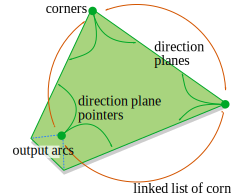
\includegraphics[width=0.8\columnwidth]{pointers.png}
%  \caption{\label{fig:pointers}
% The data structure used to build the skeleton, shown midway through the sweep}
%\end{figure}
%
%{\bf Data structures:}
%The plan data structure implicitly defines the wavefront on the sweep plane, $sp_s$. This structure is a doubly linked list of corners. Each corner has a pointer to the next corner and the previous corner (assuming counter-clockwise order) and a pointer to its previous and next edges, Fig.~\ref{fig:pointers}. Like the input polygons, the wavefront is a non intersecting collection of oriented polygons. Each corner and following corner define a single \emph{wavefront-edge}, (not to be confused with the \emph{edges} in the input) on the sweep plane. Each wavefront-edge has propagated from an edge. We calculate the wavefront for each polygon, $p$, by processing all corners, $c^p_i$. Given $c^p_i$, and the following corner, $c^p_{i+1}$, we find the associated faces with edges $e^p_{i-1}, e^p_i, e^p_{i+1}$, that is $sp^p_{i-1}, sp^p_i, sp^p_{i+1}$. We intersect the planes in which faces $sp^p_{i-1}, sp^p_i$ are embedded, and the sweep plane $sp^p_s$ to form the start of the wavefront-edge. Similarly $sp^p_{i}, sp^p_{i+1}$ and $sp^p_s$ are intersected to find the end of the wavefront-edge.
%
% At the beginning of the algorithm the data structure encodes the input. During the sweep the data structure is updated to define which corners and which portions of which edges define the bounds of the solid.
%
%A second important data structure is an priority queue that sorts events by ascending height. The strategy of our algorithm is to use a lazy evaluation of events. We fill the priority queue with a large number of potential intersection events. Wherever three or more of the unbounded faces intersect, there is a potential generalized intersection event. In addition there may be other, user-defined events (edge direction events, profile offset events or anchor events). 


\end{comment}

